Um die Frage zu beantworten wie man zwei SQL-Anfragen miteinander vergleichen kann, muss man sich die Struktur einer solchen Anfrage betrachten. Exemplarisch betrachten wir im folgenden \verb|SELECT| Anfragen. Es werden mehrere Ansätze in diesem Teil der Arbeit verfolgt, wie man die Gleichheit von zwei Anfragen zeigen kann. Offensichtlich sind zwei SQL-Anfragen semantisch äquivalent, wenn sie ebenfalls syntaktisch äquivalent sind. Interessanter sind daher Anfragen, die zunächst nicht syntaktisch deckungsgleich sind. 

Ein Ansatz besteht darin beide SQL-Anfragen einer Standardisierung zu unterziehen. Wie genau so etwas durchgeführt werden kann, wird im Folgenden noch erläutert. Dann würden wir zwei standardisierte SQL-Anfragen erhalten. Sind diese syntaktisch äquivalent, so handelt es sich um identische Anfragen. Dieser Ansatz wird uns mit einigen Problemen konfrontieren und daraus entwickeln wir einen zweiten Ansatz. Dieser versucht durch gleichartige Umformungen, die zwei Anfragen zu unifizieren (gleich zu machen). Bei diesem Ansatz würden wir also versuchen die geparsten Operatorbäume miteinander zu vergleichen. Auch diese Lösung bringt Vorteile aber auch Probleme mit sich, die im Folgenden besprochen werden.

Zu Bemerken ist hierbei, dass im folgendem Kapitel die theoretischen Grundlagen behandelt werden, die notwendig sind um zwei SQL-Anfragen auf semantische Äquivalenz zu prüfen. Dabei werden hier insbesondere auch Ideen vorgestellt, die nicht im praktischem Teil, dem Programm, auftauchen. Die Erklärung für diese Beschränkungen erfolgt in diesem Kapitel sowie im Abschnitt \ref{subsec:grenzenparser} und im Kapitel \ref{chap:praxis}.

\section{Hintergrund}

Es gibt syntaktisch unterschiedliche Anfragen, die jedoch semantisch äquivalent sind. So liefern die folgenden Anfragen die gleichen Ergebnisse obwohl sie nicht syntaktisch äquivalent sind.

\begin{verbatim}
SELECT * FROM emp e WHERE e.enr > 5
\end{verbatim}

\begin{verbatim}
SELECT * FROM emp e WHERE 5 < e.enr
\end{verbatim}

\begin{verbatim}
SELECT * FROM emp e WHERE e.enr >= 6
\end{verbatim}

Wie man leicht sieht, sind die Anfragen ähnlich. Im folgenden werden zwei Strategien besprochen, welche beide zum Ziel haben, zwei SQL-Anfragen miteinander zu vergleichen.

Neben solchen syntaktischen Varianten, kann es auch sein, dass unnötige Bedingungen aufgeschrieben werden, die das Ergebnis nur unnötig kompliziert machen. Eine Möglichkeit ist folgende Anfrage, in der offensichtlich die letzte Bedingung überflüssig ist.
\begin{verbatim}
SELECT * FROM emp e WHERE e.enr > 5 AND e.enr <> 2
\end{verbatim}

Unser Programm müsste nun erkennen, dass das Attribut \verb|enr| bereits beschränkt ist, und der Wert 2 nicht mehr auftreten kann. Das Programm, was zu dieser Arbeit entwickelt wird, kann mit solchen redundanten Eigenschaften nicht umgehen. Es wäre auch eher ein Problem für einen ``semantic checker'', da es hier nicht auf zwei verschiedene Anfragen ankommt. Hier ist bereits diese eine Anfrage in sich selbst zu kompliziert. Mit derlei Problemen beschäftigt sich das SQLLint-Projekt der Martin-Luther-Universität Halle-Wittenberg, mehr dazu im Artikel \cite{brass1} und \cite{brass2}.

Weitere Probleme sind Operatoren, die sich auf andere abbilden lassen. Man kann nie wissen, in welcher Art und Weise der Lernende die Aufgabe formulieren wird. Man betrachte dazu folgende zwei Anfragen:
\begin{verbatim}
SELECT * FROM emp e WHERE e.sal BETWEEN 10 AND 200

SELECT * FROM emp e WHERE e.sal >= 10 AND e.sal <=200
\end{verbatim}

Offensichtlich sind die Anfragen äquivalent. Dies erreichen wir im Wesentlichen, indem wir bestimmte Operatoren wie \verb|BETWEEN| abschaffen und durch äquivalente Ungleichungen mit \verb|>=| und \verb|<=| ersetzen. Ähnliches gibt es für \verb|INNER JOIN| im \verb|FROM|-Teil, mit Ersetzung durch Vergleiche im \verb|WHERE|-Teil. 

\section{Workflow}

Bereits in der Einleitung haben wir uns mit hinreichenden und notwendigen Bedingungen von semantischer Äquivalenz beschäftigt. Wir prüfen also zunächst die hinreichende Bedingung für die semantische Äquivalenz. Können beide Anfragen syntaktisch äquivalent gemacht werden, so ist klar, dass beide Anfragen auch semantisch äquivalent sind. Wir betrachten dazu zwei verschieden Ansätze. 

\subsection{Standardisierung}

Im ersten Ansatz unterziehen wir jeder Anfrage einem Standardisierungsprozess. Alle vorkommenden Variablen im FROM-Teil werden nach ihrem Namen lexikographisch sortiert und erhalten einen automatisch generierten Alias. Diese Aliase werden in allen anderen Teilen der SQL-Anfrage ersetzt durch bereits vorhandene oder eingeführt, falls vorher keine Aliase benutzt worden. Die meiste Arbeit wird im WHERE-Teil erledigt. 

Zunächst ersetzen wir syntaktische Varianten durch einheitliche Schreibweisen und entfernen syntaktische Details. Nachdem der Ausdruck des WHERE-Teils auf eine standardisierte Form (konjunktive Normalform) gebracht wurde sortieren wir den Ausdruck so, dass eine gewisse Ordnung bezüglich der Operatoren vorliegt. Weitere Anpassungen sind das Ersetzen von jedweden Unterabfragen durch äquivalente EXISTS-Unterabfragen. Im nächsten Schritt werden Verbunde (engl. Joins) kritisch untersucht und ggf. ersetzt oder vereinfacht. 

Die Operatorenvielfalt ist ein Problem, was auf zwei unterschiedliche Arten angegangen werden kann. Wir diskutieren sowohl das Hinzufügen von implizierten Formeln, als auch das Ersetzen von Formeln durch eine repräsentante Formel des gleichen Typs. Zum Abschluss werden noch GROUP BY- und ORDER BY-Ausdrücke auf ähnliche Weise angepasst.

Sind alle diese Teilschritte ausgeführt, vergleichen wir die standardisierten Anfragen auf syntaktische Äquivalenz. Bei Erfolg sind diese ebenso semantisch äquivalent.

\subsection{Elementare Transformationen}

Der zweite Ansatz ist das Anwenden von elementaren Transformationen auf einer Anfrage A um sie an eine zweite Anfrage B anzupassen. Dabei wird immer versucht Teile der Anfrage A durch Anwendung von elementaren Transformationen auf Teile von Anfrage B anzupassen. 

Zunächst wird versucht den FROM-Teil von Anfrage A anzupassen, indem wir die Anordnung der Variablennamen permutieren. Ist dies gelungen werden Aliase, die Anfrage A jetzt verwendet, in den restlichen Teilen der Anfrage A übernommen, ähnlich wie im Ansatz >>Standardisierung<<. Im WHERE-Teil wird durch sukzessives Backtracking versucht beide WHERE-Ausdrücke aneinander anzupassen. Ähnlich wir dann mit GROUP BY und ORDER BY Ausdrücken vorgegangen. Konnte das Backtracking Erfolg vermelden, so wissen wir, dass beide Anfragen semantisch äquivalent sind. 

\subsection{Erwartungen}

Wir erwarten, dass die Anpassung durch elementare Transformationen einfacher zu vollziehen ist, dafür aber eine hohe Laufzeit vorweisen wird. Dies ist zu begründen durch die exponentiell vielen Vergleiche, die beim Backtracking im worst-case auftreten können. 

Dem entgegen erwarten wir eine schnellere Laufzeit bei der Standardisierung. Dafür müssen hier deutlich mehr Teilschritte eingebaut werden und muss genau klar sein, welche Anpassungen wirklich eindeutig sind.

%\begin{verbatim}
%INPUT: QUERY Q1,Q2;
%P1 = preprocessing(Q1);
%P2 = preprocessing(Q2);
%compare(P1,P2); // possible warnings can be displayed now
%ANSWER = match(Q1,Q2);
%if ANSWER yes then
%    /* If that worked, we know both solutions are the same */
%    display success
%else 
%    if do_real_db_compare(Q1,Q2) then
%        /* now we don't know if they are the same because
%         * they couldn't be matched but test on real data 
%         * showed the correct results 
%         display may be correct
%    else 
%        /* if the real data test failed we have a proof 
%         * in form of a data set, that both querys can't be the same */
%         display fail
%    endif
%endif
%output result of compare(P1,P2)
%/* The result may show the cause of a fail or a ``may be'' solution. 
% * It can provide hints so that the student can improve.
% * Even if the solution was correct i.e. it was matched with the sample solution, 
% * it may be that the students solution contained unnecassary joins, or formulas. */
%\end{verbatim}

\subsection{Preprocessing}
\label{subsec:preprocessing}

Im Abschitt >>Forschungsstand<< haben wir bereits einige Lernplattformen/ -projekte zum Thema SQL kennen gelernt. Viele dieser Plattformen möchten dem Lernenden genügend Feedback beim Lernprozess geben. Dies ist nicht nur sinnvoll, damit der Student schneller auf korrekte Lösungen stößt, sonder auch, weil die Standardhinweise eines SQL-Systems meist nur auf syntaktische Fehler hinweisen. Einen großen Beitrag zur Verbesserung von Fehlermeldungen hat das Projekt SQLLint vorzuweisen, da es Fehlermeldungen und Hinweise konkreterer Natur ausgibt. Hervorzuheben ist noch einmal, dass es sich hierbei um semantische Fehlermeldungen handelt. Schon nach kurzer Einlernzeit sinkt die Anzahl syntaktischer Fehler bei Lernenden. Dafür machen diese mehr semantische Fehler, was um so schlimmer ist, da bisher kaum oder keine Warnhinweise für solche Fehler existierten. 

Dennoch sollen in dieser Arbeit zwei SQL-Anfragen verglichen werden. Wir können hier also nicht alle Ideen des SQLLint übernehmen. Egal ob das Matchen der Musterlösung und der Lösung des Lernenden gelingt oder nicht, wir möchten dem Lernenden ein Feedback geben, an dem er idealerweise sehen kann, warum das Matching nicht gelungen ist. Wir können dabei, wie bereits erwähnt, nicht an die Komplexität des SQLLint anknüpfen. Stattdessen werden wir uns eines einfachen Sammelns von Metainformationen der SQL-Anfrage bedienen. Diese sammeln wir bevor die zwei Anfragen durch Folgeschritte angepasst oder verändert werden. Am Ende des Matchingsversuchs sollen die Metainformationen der zwei Anfragen verglichen werden und dem Lernenden soll ein Feedback gegeben werden. Konnte keine Übereinstimmung der zwei Anfragen erreicht werden, so können die Metainformationen dem Lernenden Anhaltspunkte für eine richtige Lösung geben. Konnten die Anfragen unifiziert werden, so sind die Metainformationen dennoch von Interesse. Es könnte sein, dass der Lernende eine unnötig komplexe Lösung eingesandt hat, die sich durch Anpassungen vereinfachen ließe. So kann der Lernende potentiell auch aus einer korrekten Lösung noch etwas lernen.

Wir möchten für jede SQL-Anfrage ein Preprocessing vor der eigentlichen Bearbeitung vorschalten, was im Wesentlichen folgende Punkte beinhalten soll:

\begin{itemize}
\item Anzahl der JOIN Bedingungen
	\begin{itemize}
	\item Anzahl von OUTER/ INNER Joins
	\end{itemize}
\item Anzahl atomarer Formeln im \verb|WHERE|-Teil
\item Anzahl atomarer Formeln im \verb|HAVING|-Teil
\item Anzahl Tabellen in \verb|FROM|-Teil
\item Anzahl Attribute im \verb|SELECT|-Teil *
\item existiert ein \verb|DISTINCT|
\item existiert ein \verb|GROUP BY| *
	\begin{itemize}
	\item wenn ja, tauchen Variablennamen und Aggregationsfunktionen auch im SELECT-Teil auf?
	\end{itemize}	 
\item existiert ein \verb|HAVING BY|
\item existiert ein \verb|ORDER BY| und ist es notwendig? (\verb|ORDER BY ... ASC|) *
\item Tiefe des Parserbaums kann Aufschluss über unnötige Klammerung geben. Siehe dazu Abschnitt >>Wie funktioniert der Parser<<
\end{itemize}

Unterscheiden sich Musterlösung und Lösung des Studenten in den mit * markierten Punkten ist es extrem unwahrscheinlich, dass beide Lösungen die gleichen Tupel zurückliefern würden. Hier möchten wir im Vorfeld dem Lernenden eine Warnung anzeigen, dass er höchstwahrscheinlich etwas vergessen hat. Alle anderen Punkte werden im Anschluss an die eigentliche Analyse der Anfragen abgeglichen. So sind etwa folgende Meldungen denkbar:

\begin{itemize}
\item ``The sample solution contains two joins but your solution does not contain any join.''
\item ``Your solution is correct but the sample solution contains two less atomar formulas (formula1, formula2).''
\item ``Your solution is correct but the sample solution does not contain DISTINCT. Reconsidder if it is really necessary.''
\end{itemize}

Zusammenfassend kann man Folgendes sagen: Das Preprocessing wird direkt nach dem Parsen einer SQL-Anfrage durchgeführt. Es sammelt Metainformationen über die Anfrage. Da wir zwei Anfragen vergleichen, werden diese Metainformationen einzeln für jede Anfrage gespeichert. Dann beginnen wir mit dem zweiten Schritt, dem Angleichen der SQL-Anfragen. Dazu verwenden wir Strategien, die in folgenden Kapiteln besprochen werden.

Egal ob die Ergebnisse im zweiten Schritt erfolgreich waren oder nicht, wir geben danach einen Vergleich der Metainformationen aus. Beispiele wurden eben bereits genannt. Das soll dem Lernenden bei falschen Lösungen Anhaltspunkte geben, wie eine richtige Lösung aussehen könnte. Bei einer korrekten Lösung, können solche Hinweise trotzdem nützlich sein, denn die Anfrage des Lernenden kann trotz Korrektheit zu lang bzw. kompliziert sein. Dies würde bei einem Vergleich der gesammelten Metainformationen deutlich werden.

\section{Standardisierung von SQL-Anfragen}

Zunächst verfolgen wir den Ansatz zwei SQL-Anfragen zu vergleichen, indem wir sie standardisieren. Die Kriterien der Standardisierung werden im Detail behandelt. Standardisiert man die Musterlösung, als auch die Lösung des Lernenden nach den gleichen Kriterien, so kann man danach durch einen einfachen Stringvergleich auf die Äquivalenz schließen. 

\subsection{Entfernen von syntaktischen Details}

Das Entfernen von syntaktischen Details übernimmt zum großen Teil bereits der Parser. Er entfernt unnötige Leerzeichen, Kommentare sowie unnötige Klammern. Aufgrund der Arbeitsweise des Parsers gibt es allerdings Situationen, in dem der Parser scheinbar nicht alle unnötigen Klammern entfernt. Wie im Abschnitt >>Verwendeter Parser<< erläutert wird, sind die geparsten Bäume nicht binär. Ein Baum wie in Abbildung \ref{baum1} zu sehen, ist daher zu vermeiden. 

Der Parser hilft allerdings dabei die SQL-Anfrage in einer Datenstruktur zu überführen, die frei von allen syntaktischen Details ist. Dazu gehören Leerzeichen, Tabs, Zeilenumbrüche und Groß-/ Kleinschreibung von Schlüsselwörtern.

\subsection{FROM-Teil}
\label{subsec:from}

Wir beginnen mit der Betrachtung der \verb|FROM|-Klausel. Da die Reihenfolge der Spaltennamen im \verb|SELECT|-Teil oft von der Aufgabenstellung vorgeschrieben ist, wird diese auch nicht verändert.

Im \verb|FROM| Teil werden zunächst alle auftretenden Tabellennamen lexikographisch sortiert. Danach werden automatische Aliase erzeugt. Sind bereits Aliase vergeben wurden, so werden diese ebenfalls durch die automatischen Aliase ersetzt. Eine Hashtabelle speichert frühere Zuweisungen, damit im \verb|SELECT|-, \verb|WHERE|-, \verb|GROUP BY|- und \verb|ORDER BY|-Teil die Aliase ebenfalls korrekt ersetzt werden.

Hatten die vorkommenden Tabellen im \verb|FROM|-Teil keinen Alias wird nur der küsntliche Alias eingeführt.

\begin{figure}
Eingabe: \\\verb|SELECT e.id, e.name, d.region FROM emp e, dep d WHERE e.depid = d.id|\\

Anpassung: \\\verb|SELECT a2.id, a2.name, a1.region FROM dep a1, emp a2 WHERE a2.depid = a1.id|\\
\caption{Beispiel: Umwandlung des FROM-Teils einer SQL-Anfrage}
\end{figure}

\subsection{WHERE-Teil}

Aufgrund der Eigenheiten des ZQL-Parsers ist es möglich, dass eine unnötige Klammerung nicht entfernt wird. Beispiele dafür sind im Abschnitt >>ZQL-Parser<< zu finden. Es ist daher wünschenswert eine Normalform des \verb|WHERE|-Teils zu erreichen. In diesem Fall wurde die konjunktive Normalform (KNF) gewählt.


\subsubsection{Entfernung unnötiger Klammerungen}

Ein Ausdruck \verb|((a > 5)  and ((b > 5) and (c > 5)))| enthält unnötige Klammern, da der Operator \verb|and| als Operand von einem weiteren \verb|and| vorkommt. Folgender Ausdruck ist äquivalent: \verb|((a > 5)  and (b > 5) and (c > 5))|. Diese spezielle Form der Klammerung entsteht aus der Tatsache, dass der ZQL-Parserbaum nicht binär ist und beide eben genannten Beispiele nicht den gleichen Baum beschreiben. Als ersten Schritt in Richtung KNF möchten wir solche unnötigen Klammern entfernen. 

Es ist daher wünschenswert, wenn ein Operator X einen Ausdruck als Kindknoten besitzt, indem X ebenfalls der Operator ist, den Operator X im Kindknoten zu eliminieren. Alle Kinder vom eliminierten Kindknoten an hängen wir nun an den verbleibenden Operatorknoten X. Damit hätte man den Ausdruck vereinfacht, da die assoziative Klammerung wegfällt. Wir nennen dieses Vorgehen im Folgenden Operatorkompression. Verbildlicht wird dieser Vorgang im Abschnitt >>Funktionsweise des Parsers<<.

Gegeben sei der ZQL-Parsebaum $B=(V,E)$. Es sei $child(v) = \{ w : w\in V \wedge (v,w)\in E\}$, also die Menge aller Kindknoten von $v$. Gibt es einen Knoten $w\in child(v)$ mit $v=w$, so wird Knoten $w$ eliminiert und alle Kindknoten von $w$ werden zu Kindknoten von $v$, also $child(v) = child(v) \cup child(w)$. 
$E=E\backslash \{ (w,x) : x\in child(w)\} \cup \{(v,x) x\in child(w)\}$ und $V=V\backslash \{w\}$.

Im Sinne des Vergleiches der Komplexität der Musterlösung mit der Komplexität der Lösung des Lernenden ist es sinnvoll zu speichern, ob und wie oft eine solche Operatorkompression durchgeführt werden musste.

\subsubsection{NOT auflösen}

Im nächsten Schritt möchten wir auftretende \verb|NOT|-Operatoren entfernen. Dies geschieht, indem der Operator \verb|NOT| im Parserbaum nach unten geschoben wird. Dabei werden die \textit{DE MORGAN}-Regeln angewendet. 

\begin{tabular}{ll}
Eingabe: & Umwandlung Teil 1:\\
\verb|not ((a > 5)  and ((b > 5) or (c > 5)))| & \verb|(not(a > 5) or not((b > 5) or (c > 5)))|\\
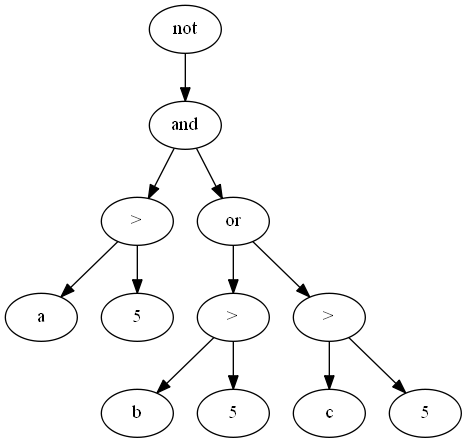
\includegraphics[scale=0.5]{Bilder/not_graph1.png} & 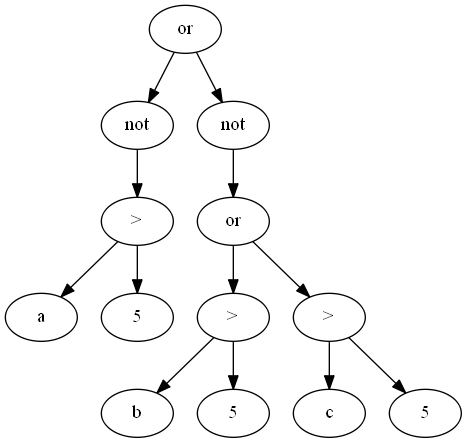
\includegraphics[scale=0.5]{Bilder/not_graph2.png}\\
\end{tabular}

\begin{tabular}{ll}
Umwandlung Teil 2: & Umwandlung Teil 3:\\
\verb|((a <= 5) or (not(b > 5) and not(c > 5)))| & \verb|((a <= 5) or ((b <= 5) and (c <= 5)))|\\
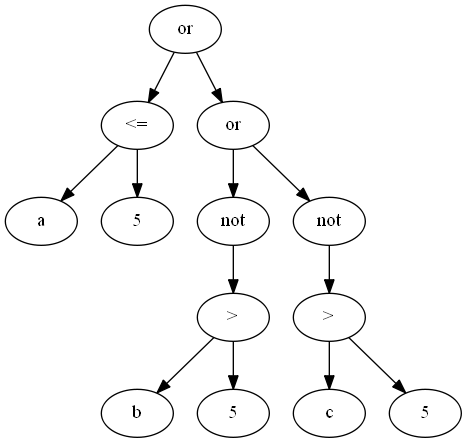
\includegraphics[scale=0.5]{Bilder/not_graph3.png} & 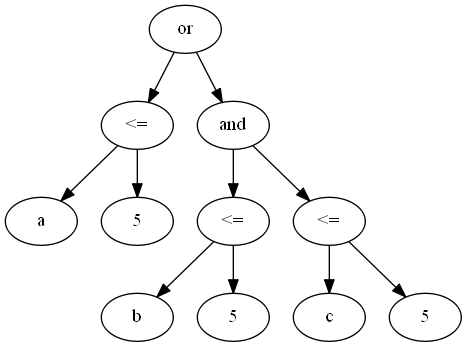
\includegraphics[scale=0.5]{Bilder/not_graph4.png}\\
\end{tabular}


\subsubsection{Anwenden des Distributivgesetzes}

Im letzten Schritt haben wir die Formel \verb|((a <= 5) or ((b <= 5) and (c <= 5)))| erhalten. Durch Anwenden des Distributivgesetzes können wir diese Formel im letzten Schritt umformen zu: \verb|((a <= 5) or (b <= 5)) and ((a <= 5) or (c <= 5))|

\subsection{Ersetzung von syntaktischen Varianten}

Um eine Anfrage zu standardisieren müssen wir den syntaktischen Zucker entfernen. Dies geschieht, indem man nur eine syntaktische Schreibweise anerkennt und alle anderen Schreibweisen in die zulässige umgewandelt. 

Mit dem Operator \verb|BETWEEN| testen wir ob ein gegebener Ausdruck zwischen zwei Werten, upper und lower, befindet. Wir schreiben den Ausdruck \verb|e BETWEEN upper AND lower| äquivalent um, in dem wir nur Vergleichsoperatoren benutzten. \\Unser Ausdruck lautet dann: \verb|e >= upper AND e <= lower|.

Der Operator \verb|IN| prüft, ob ein gegebener Ausdruck einen bestimmten Wert, aus einer Liste, zugewiesen ist. Die Liste kann dabei als Unterabfrage oder als Liste von Konstanten beschrieben werden. Handelt es sich um eine Liste von Konstanten, so können wir \\\verb|e IN (const1, const2, ..., constn)| ersetzen, in dem wir prüfen ob \verb|expression| einen der konstanten Werte annimmt. Wir verknüpfen also $n$ Vergleiche disjunktiv miteinander. Wir erhalten dadurch: \verb|e = const1 OR e = const2 OR ... OR e = constn|.

Ähnlich dazu verhält sich der Operator \verb|ALL|. Er tritt in folgender Form auf:\\
\verb|operand comparison_operator ALL (subquery)|. Dabei kann \verb|subquery| auch eine Liste von Konstanten sein. Es wird in jedem Fall geprüft ob der Operand und jedes der Listenelemente in der Vergleichsrelation enthalten ist. Haben wir als \verb|subquery| eine Liste von Konstanten, so ist dies äquivalent mit dem paarweisen Vergleich von \verb|operand| und jedem Listenelement. Diese $n$ Vergleiche werden dann konjunktiv verknüpft, also: \\
\verb|operand operator elem1 AND ... AND operand operator elemn|. 
Diese syntaktische Anpassung ist nicht im Programm enthalten, da der ZQL-Parser keine Listen unter \verb|ALL| versteht.

Der Operator \verb|ANY| ist beinahe äquivalent zu \verb|ALL| mit dem Unterschied, dass die entstandene Liste der Vergleiche nicht konjunktiv, sondern disjunktiv verknüpft wird.

Befindet sich im \verb|WHERE|-Teil eine \verb|EXISTS|-Unterabfrage, so können wir den \verb|SELECT|-Teil dieser Unterabfrage vereinfachen. Da wir nur wissen wollen ob es Ergebnistupel aus der Unterabfrage gibt, ist es nicht notwendig bestimmte Spalten aus dieser Unterabfrage zu abzufragen, da wir diese in der Oberanfrage nicht verwenden oder brauchen. Daher ersetzen wir den \verb|SELECT|-Teil von \verb|EXISTS|-Unterabfragen zu:\verb|SELECT 1|. Ein Beispiel dieser Umwandlung ist in Abbildung \ref{fig:exists_ex1} zu sehen.

\begin{figure}[h]
\begin{verbatim}
SELECT e.sal FROM emp e WHERE EXISTS (
    SELECT expression FROM dept d 
    WHERE e.deptno = d.deptno )
    
SELECT e.sal FROM emp e WHERE EXISTS (
    SELECT 1 FROM dept d 
    WHERE e.deptno = d.deptno )
\end{verbatim}
\caption{Umwandlung des SELECT-Teils einer EXISTS-Unterabfrage}
\label{fig:exists_ex1}
\end{figure}


%\begin{figure}[h]
%\begin{tabular}{ccl}
%\verb|A BETWEEN B AND C| & $\to$  & \verb|A >= B AND A <= C|\\
%\verb|SELECT ALL| & $\to$ & \verb|SELECT|\\
%\verb|ORDER BY VAR ASC| &  $\to$ & \verb|ORDER BY VAR|\\
%\verb|A IN ('X', 'Y', 'Z')| & $\to$ & \verb|A = 'X' OR A = 'Y' OR A='Z'|\\
%\verb|EXISTS (SELECT A,B,C ...)| & $\to$ & \verb|EXISTS (SELECT 1 ...)|\\
%\end{tabular}
%\caption{Entfernen von syntaktischen Varianten}
%\end{figure}

\subsubsection*{Unteranfragen}

Es ist bekannt, dass sämtliche Typen von Unteranfragen eliminiert oder durch \verb|EXISTS|-Anfragen ersetzt werden können. Streng genommen handelt es sich hier zwar um mehr als nur eine syntaktische Variante, aber dennoch wollen wir das Ersetzen von Unteranfragen in diesem Abschnitt betrachten.

Wir behandeln in diesem Abschnitt nur echte Unterabfragen, das heißt die Unterabfrage darf keine Liste von Konstanten sein. Ist die Unterabfrage eine Liste, \mbox{z. B.} bei \verb|ALL, ANY| oder \verb|IN| gehen wir vor, wie im vorherigen Abschnitt beschrieben.

\subsubsection*{ALL-Unterabfragen}

\verb|ALL|-Unterabfragen haben immer das Muster: \verb|operand comparison_operator ALL (subquery)|. Dabei handelt es sich bei \verb|comparision_operator| um \verb|{=,<>,>,<,>=,<=}|. Die Unterabfrage \verb|subquery| liefert eine Liste von Attributen. Dann wir so verfahren wie bereits im letzten Abschnitt erklärt. Unser Ziel ist es, diese Unterabfrage, wenn möglich, zu ersetzen durch eine \verb|EXISTS|-Unterabfrage. Um diese Umwandlung nachzuvollziehen, wandeln wir zunächst die Unterabfrage mit \verb|ALL| in eine Unterabfrage mit \verb|ANY| um. Dazu ersetzen wir den \verb|comparison_operator| mit seinem gegenteiligem Operator. Folgende Paare sind jeweils voneinander gegenteilige Operatoren: \verb|{ {<,>=}, {>,<=}, {=,<>} }|. Danach ersetzen wir \verb|ALL| mit \verb|ANY| und kapseln die gesamte Unterabfrage mit einem \verb|NOT|. 

%\begin{figure}
\begin{lstlisting}[mathescape]
WHERE $t_1$ comparison_operator ALL (
	SELECT $t_2$
	FROM $R_1$ $X_1$, ..., $R_n$ $X_n$
	WHERE ($\varphi$)
)

Geschrieben als ANY-Unterabfrage:
WHERE NOT( $t_1\ $opposite(comparison_operator$)$ ANY (
	SELECT $t_2$
	FROM $R_1$ $X_1$, ..., $R_n$ $X_n$
	WHERE ($\varphi$) ) 
)
\end{lstlisting}

Diese \verb|ANY|-Unterabfrage können wir nun in eine \verb|EXISTS|-Unterabfrage transformieren. Wie das genau durchgeführt wird, behandeln wir jetzt im nächsten Abschnitt.

%\caption{Umwandeln von \verb|ALL|- in \verb|ANY|-Unterabfrage}
%\label{fig:all_ex2}
%\end{figure}

\subsubsection*{ANY/ SOME-Unterabfragen}

Da \verb|SOME| und \verb|ANY| äquivalente und synonyme Schlüsselworte sind betrachten wir im Folgenden nur \verb|ANY|-Unterabfragen. Eine solche Unterabfrage kann in eine \verb|EXISTS|-Unterabfrage umgewandelt werden. Dazu verknüfen wir den Vergleichsoperator mitsamt linken Operanden konjunktiv mit dem \verb|WHERE|-Teil der Unterabfrage. Als rechten Operanden wählen wir das Attribut, welches sich im \verb|SELECT|-Teil der Unterabfrage befindet. Die Umwandlung findet also nach folgendem Muster statt:

\begin{lstlisting}[mathescape]
WHERE $t_1\ $comparison_operator ANY (
	SELECT $t_2$
	FROM $R_1$ $X_1$, ..., $R_n$ $X_n$
	WHERE ($\varphi$) 
) 

Geschrieben als EXISTS-Unterabfrage:
WHERE EXISTS( 
	SELECT $t_2$
	FROM $R_1$ $X_1$, ..., $R_n$ $X_n$
	WHERE ($\varphi$ 
	AND $t_1$ comparison_operator $t_2$ )
)
\end{lstlisting}

Wie wir am Ergebnis der Umwandlung erkennen, verstößt $t_2$ im \verb|SELECT|-Teil der \verb|EXISTS|-Unterabfrage bereits gegen unsere Konvention, die einige Seiten vorher getroffen wurde. Es empfiehlt sich daher, die Normierung des \verb|SELECT|-Teils von \verb|EXISTS|-Unterabfragen erst nach dem Umwandeln von Unterabfragen durchzuführen.


\subsubsection*{IN-Unterabfragen}

Das Schlüsselwort \verb|IN| ist lediglich ein Synonym für \verb|= ANY|. Diese Unterabfragen sind daher ein Spezialfall der, bereits betrachteten, \verb|ANY|-Unterabfragen.

\subsubsection*{Voraussetzungen}

Alle, eben genannten, Umwandlungen können nur durchgeführt werden, wenn bestimmte Bedingungen erfüllt sind.

\begin{enumerate}
\item Alle Tupelvariablen, die in $t_1$ vorkommen, müssen sich unterscheiden von allen $X_i$. Erreicht wird dies ggf. durch Umbenennung der $X_i$, da diese nicht für die eigentliche (Ober)anfrage wichtig sind.
\item Wenn $t_1$ Attributreferenzen $A$ ohne Tupelvariable enthält, dann dürfen die $R_i$ kein Attribut $A$ haben. Erreicht wird dies, indem ggf. die Tupelvariable eingeführt wird.
\item Die Unteranfrage für $t_2$ darf keine Nullwerte liefern. 
\end{enumerate}

wir haben im Abschnitt \verb|FROM|-Teil bereits festgelegt, dass sämtliche Aliase der Tupelvariablen automatisch erzeugt werden. Dies gilt in natürlicher Weise auch für Unterabfragen. Der Prozess erstreckt sich von Einführung von Aliasen, falls vorher keine Vorhanden waren, bis hin zur Umbenennung bereits vorhandener Aliase, sodass niemals identische Aliase innerhalb einer SQL-Anfrage vorkommen können. Damit erfüllen wir bereits die Bedingung 1 und 2. 

Da es nicht entscheidbar ist, ob eine Unterabfrage \verb|NULL|-Werte liefern kann, vereinfachen wir das Entscheidungskriterium dafür. Wenn eine der zugehörigen Spalten in $t_2$ so definiert ist, dass \verb|NULL|-Werte laut Definition des Datenbankschemas erlaubt sind, so gehen wir davon aus, dass die Unterabfrage \verb|NULL|-Werte liefern wird. Wir wandeln in einem solchen Fall die Unterabfrage nicht um.

\subsubsection{Andere Unteranfragen}

Ungewöhnliche Unterabfragen, wie \mbox{z. B.} Unterabfragen unter \verb|FROM| werden hier nicht betrachtet. Im Allgemeinen werden solche Unterabfragen kaum gebraucht und machen die Anfrage meist nur viel komplexer als notwendig.

\subsection{Operatorenvielfalt}

Im folgenden Abschnitt soll geklärt werden wie mit verschiedenen Schreibweisen von ein- und demselben Ausdruck umgegangen werden soll. Betrachtet man sich \mbox{z. B.} \verb|A > 5| ist dieser Ausdruck äquivalent mit \verb|5 < A|. Wenn wir wissen, dass \verb|A| ein ganzzahlige Variable ist, dann sind auch folgende Äquivalenzen wahr: \verb|A >= 6| sowie \verb|6 <= A|. Wir betrachten nun zwei verschiedene Ansätze um mit diesem Problem umzugehen. Der erste Ansatz beschäftigt sich damit, alle implizierten Schreibweisen mit in die Formel aufzunehmen. Damit stellt man sicher, dass sich alle korrekten Schreibweisen einer Formel in der Anfrage befinden. Der zweite Ansatz beschäftigt sich damit, nur bestimmte Schreibweisen zuzulassen und alle anderen durch die zulässigen zu ersetzen.

\subsubsection{Analyse der unterschiedlichen Operatoren}

Wir unterscheiden im wesentlichen zwei Arten von Operatoren. Zum einen Operatoren, bei denen wir die Operanden in beliebiger Reihenfolge anordnen können. Wir nennen diese Operatoren, kommutative Operatoren. Dies sind \verb|{ =, AND, OR, +, *}|. Alle anderen Operatoren sind demnach nicht kommutativ, da wir die Reihenfolge der Operanden nicht ändern können, ohne den Ausdruck zu verfälschen. Zu dieser Gruppe von Operatoren zählen insbesondere \verb|{ >=, >, <, <=, -, /, }|. Eine dritte Gruppe bilden unäre Operatoren, die nur ein Operanden kennen. Diese Gruppe ist aber im Sinne der Anordnung uninteressant, da wir hier keine mehrdeutig aufgeschrieben Varianten haben.

Ziel ist es, nach wie vor, eine gewisse Ordnung zu definieren, so dass nach der Standardisierung semantisch gleiche Anfragen auch syntaktisch gleich sind. Betrachten wir nun einen Ausdruck mit einem Operator $op$ und $n$ Operanden bezeichnet als $child_i$. Ist $op$ ein kommutativer Operator, so können wir die Operanden $child_i$ beliebig anordnen ohne den Sinn des Ausdrucks zu verändern. Dies tun wir, in dem wir eine bestimmte Sortierreihenfolge etablieren. Diese finden wir im späteren Abschnitt \ref{subsec:sort}.

Diese Sortierung ist nicht möglich, wenn $op$ nicht kommutativ ist. In einem solchen Fall müssen wir also die äquivalenten Schreibweisen des Ausdrucks mit in unsere Formel aufnehmen und konjunktiv mit dem Originalausdruck verknüpfen. Im folgenden Beispiel sei angenommen, dass $a$ vom Typ \verb|INT| ist.
Zu beachten ist, dass im Beispiel der Operator $>$ nicht kommutativ ist und daher all seine weiteren Schreibweisen hinzugefügt werden müssen.

\begin{verbatim}
Eingabe:
SELECT * FROM emp e WHERE e.sal > 1000

Vervollständigte Form:
SELECT * FROM emp e WHERE e.sal > 1000 AND 1000 < e.sal AND e.sal >= 1001 AND 1001 <= e.sal
\end{verbatim}

Zu beachten ist weiterhin, dass wir nach der Umformung vier anstatt einer Formel haben. Diese Formeln müssen auch eine gewissen Ordnung unterzogen werden, da der übergeordnete Operator \verb|AND| wiederum kommutativ ist. Die Art dieser Ordnung wird im Abschnitt \ref{subsec:sort} beschrieben.

Wir möchten im folgenden zunächst diskutieren, wie wir diese implizierten Formeln hinzufügen können. Im Anschluss daran diskutieren wir, wie eine Sortierordnung aussehen kann.

\subsubsection{Hinzufügen implizierter Formeln}

Wie bereits im vorherigen Beispiel ersichtlich, sind die hinzugefügten Formeln redundant und tragen nicht effizient zur Beschleunigung der Anfrage bei. Es soll hier lediglich sichergestellt werden, dass alle möglichen äquivalenten Formeln auftreten, da wir nicht wissen, was der Lernende für einen Repräsentanten der Formeln wählen wird. Weiterhin muss bemerkt werden, dass dadurch die gesamte SQL-Anfrage enorm aufgebläht wird. Es ist daher unbedingt wichtig, die Originalanfrage zu speichern. Weiterhin muss das Programm eine Verbindung zwischen den Formeln der Originalanfrage und den Formeln der veränderten, aufgeblähten Anfrage herstellen. Dem Lernenden soll in einem Feedback nur Fehler in der Originalanfrage aufgezeigt werden. Da intern aber mit der aufgeblähten Anfrage gearbeitet wird, muss beim Auftreten eines Fehlers oder Hinweises nachgeschlagen werden, von welchem Teil der Originalanfrage der Teil entstammt, der jetzt den Fehler auslöst.

Im Folgenden listen wir Mengen $M_i$ von Ausdrücken. Finden wir in der zu bearbeitenden SQL-Anfrage eine Formel $f$, die auf einen Ausdruck $a\in M_i$ passt, dann verknüpfen wir alle Ausdrücke $\{b : b\in M_i \wedge b \neq a\}$ konjunktiv mit $f$. Dabei sind alle Variablennamen $A,B,C$ keine (komplexen) Ausdrücke. Es handelt sich also jeweils um Blattknoten im Parserbaum. Ferner bezeichnen wir $X,Y$ als numerische Konstanten.\\

\begin{tabular}{ll}
$M_1$ & $\{\ A=B-C\ ,\ C=B-A\ ,\ B=A+C\ \}$\\
$M_2$ & $\{\ A=B\cdot C\ ,\ C=A / B\ ,\ B=A / C\ \}$\\
$M_3$ & $\{\ A>B-C\ ,\ C>B-A\ ,\ B<A+C\ \}$\\
$M_4$ & $\{\ A<B-C\ ,\ C<B-A\ ,\ B>A+C\ \}$\\
$M_5$ & $\{\ A>B, B<A \}$\\
$M_6$ & $\{\ A\geq B, B\leq A \}$\\
$M_7$ & $\{\ A>X, A\geq X+\mathit{adjust}(A) \}$\\
$M_8$ & $\{\ A<X, A\leq X-\mathit{adjust}(A) \}$\\

\end{tabular}

Beim Vergleich mit $>$ und $<$ ist es wichtig zu wissen, wie viel Nachkommastellen die numerischen Variablen $A$ und $B$ besitzen. Es sei $\mathit{places}(A)$ die Anzahl der Nachkommastellen der Zahl $A$. Dann bezeichnen wir mit $\mathit{adjust}(A) = 1 / (10^{\mathit{places}(A)})$, einen angepassten Wert, der sich nach der Stelligkeit der Variable A richtet.

Betrachten wir als Beispiel ein Attribut \verb|salery|, welches als \verb|NUMERIC(4,2)| definiert ist. Wir wissen also, dass \verb|salery| zwei Nachkommastellen hat. Betrachten wir nun die Aussage \verb|salery >= 5|.
Wir haben auf einer Seite eine Variable (\verb|salery|) und auf der anderen Seite eine numerische Konstante (\verb|5|). Dieses Muster passt also auf $M_7$ und auf $M_6$. In $M_7$ heißt es $A\geq X+\mathit{adjust}(A)$. Bezogen auf unser Beispiel ist \verb|A=salery| und \verb|x+adjust(salery)=5|. Wir berechnen also: 
$$\mathit{adjust}(\mathit{salery}) = 1 / (10^{2}) = 1/100 = 0,01$$
Wir erhalten also \verb|x=4,99|, weil \verb|x+0,01=5|. Somit ergänzen wir unsere Ausgangsformel \verb|salery >= 5| konjunktiv mit \verb|salery > 4,99|. Weiterhin muss jetzt wegen $M_6$ \verb|5 <= salery| und wegen $M_5$ \verb|4,99 < salery| hinzugefügt werden.

Finden wir Ausdrücke mit $>,<,\leq,\geq$, welche als Argumente Variablen oder Konstanten haben, so unterscheiden wir also grundsätzlich drei Fälle.

Fall 1 $(M_5,M_6)$: Beide Operanden sind Variablen oder Konstanten. In diesem Fall ergänzen wir nur den jeweils symmetrischen Operator. Da beide Operanden Variablen sind, macht es weniger Sinn jeweils $\leq,\geq$ oder $<,>$ zu ersetzen, da normalerweise ein künstliches hinzufügen eines Summanden auf einer Seite, die Anfrage unnatürlich aussehen lässt. Es ist aber auch kein Problem diese Ersetzungen auch durchzuführen, wenn beide Operanden Variablen sind. Die Anfrage wird dann natürlich noch weiter künstlich aufgebläht.

Fall 2 $(M_7,M_8)$: Einer der beiden Operanden ist eine numerische Konstante und der andere ist eine Variable. In diesem Fall fügen wir alle implizierten Gleichungen hinzu, also insbesondere die Operatoren $\leq,\geq,<,>$. Zu beachten ist hier, dass nicht nur Gleichungen der Form $A>X$ dazu führen, dass alle Ausdrücke von $M_7$ hinzugefügt werden. Auch wenn eine Gleichung der Form $Var1\geq 5.2$ auftaucht, werden Ersetzungen durchgeführt. Diese Gleichung passt auf das Muster $A\geq X+\mathit{adjust}(A)$. Angenommen $Var1$ hat maximal eine Nachkommastelle, so würden dann folgende Gleichungen impliziert werden: $\{\ Var1>5.1\ ,\ 5.1<Var1\ ,\ 5.2 \leq Var1\ \}$.

Fall 3: Beide Operanden sind numerische Konstanten. In dem Fall wird die logische Aussage ausgewertet und durch ihren Wahrheitswert ersetzt [0,1].

Sind durch die hinzugefügten Terme nun arithmetische Ausdrücke entstanden, die nur noch numerische Konstanten enthalten, so werden diese Ausdrücke ausgewertet.

In einem anschließenden Schritt werden arithmetisch/logische Ausdrücke ausgewertet und durch ihre Ergebnis ersetzt. Dieser Schritt muss BOTTOM-UP geschehen, damit man auch mehrere Ersetzungen nach oben, im Parserbaum, weiterreicht. Haben wir am Ende einen SQL-Ausdruck dessen \verb|WHERE|-Teil aus \verb|false| besteht, dann haben wir eine Anfrage gefunden, die immer das leere Ergebnis liefern wird. In diesem Fall müssen wir natürlich eine Fehlermeldung ausgeben.

\subsubsection{Beschränkung der Operatorenvielfalt}

Ein weiterer Ansatz das Problem der äquivalenten Formeln anzugehen ist es, bestimmte Operatoren zu >>verbieten<<. Das soll bedeuten, wir definieren verbotene Operatoren, welche am Ende der Umwandlungen nicht mehr in der SQL-Anfrage vorkommen dürfen. Dies wird erreicht, indem wir jeden verbotenen Operator umwandeln in einen nicht-verbotenen Operator. Das Prinzip ähnelt dem eben Vorgestellten. Wir betrachten wieder die Mengen $M_i$. Des Weiteren hat jede Menge $M_i$ einen Repräsentanten $r(M_i)$. Finden wir nun in der zu bearbeitenden Anfrage eine Formel $f$, die auf eine der Ausdrücke $a\in M_i$ passt, so ersetzen wir $f$ mit $r(M_i)$. Folgende Tabelle soll die Mengen und deren Repräsentanten beschreiben.

Im folgenden sind alle Variablennamen $A,B,C$ keine (komplexe) Ausrücke. Es handelt sich also jeweils um Blattknoten im Parserbaum. Ferner bezeichnen wir $X,Y$ als numerische Konstanten.\\

\begin{tabular}{lll}
$i$ & $M_i$ & $r(M_i)$ \\
$1$ & $\{\ A=B-C\ ,\ C=B-A\ ,\ B=A+C\ \}$ & $B=A+C$\\
$2$ & $\{\ A=B\cdot C\ ,\ C=A / B\ ,\ B=A / C\ \}$ & $A=B\cdot C$\\
$4$ & $\{\ A>B-C\ ,\ C>B-A\ ,\ B<A+C\ \}$ & $A>B-C$ \\
$5$ & $\{\ A<B-C\ ,\ C<B-A\ ,\ B>A+C\ \}$ & $A<B-C$\\
$6$ & $\{\ A>B, B<A \}$ & $A>B$\\
$7$ & $\{\ A\geq B, B\leq A \}$ & $A\geq B$\\
$8$ & $\{\ A>X\ ,\ X<A,A\geq X+\mathit{adjust}(X)\ ,\ X\leq A - \mathit{adjust}(X)\ \}$ & $A>X$\\
\end{tabular}

Im Folgenden soll ein Beispiel die Prozedur verdeutlichen.\\

Es sei unsere Ausgangsanfrage: \begin{verbatim}SELECT * FROM testtable WHERE X = 6 - Y\end{verbatim}

Die Formel $X=6-Y$ finden wir in $M_1$ in Form von $A=B-C$. Wir ersetzen nun also $X=6-Y$ mit dem Repräsentanten von $M_1$, und wir bekommen: \begin{verbatim}SELECT * FROM testtable WHERE 6 = X + Y\end{verbatim}

Ein Problem bei der Verwendung von Repräsentanten durch Einschränkung der Operatorenvielfalt ist, dass es zu überlappenden Mengen kommen kann. Damit ist gemeint, dass ein Ausdruck auf mindestens zwei Mengen $M_i$ und $M_j$ mit $i\neq j$ passt. Man muss sich in einem solchen Fall fragen, welchen Ausdruck man als Repräsentanten wählt. Es gibt mehrere Arten mit diesem Problem umzugehen. Auf der einen Seite könnte man die Mengen so umgestalten, dass alle Mengen $M_i$ jeweils, paarweise disjunkte Mengen darstellen, dann käme es zu keiner derartigen Überlappung. Zum anderen könnte man eine Ordnung vorschreiben. Würde ein Ausdruck $expr$ auf die Mengen $M_i$ und $M_j$ mit $i\neq j$ passen wählen wir den Repräsentanten $r(M_i)$ genau dann, wenn $i < j$, ansonsten wählen wir $r(M_j)$.

In unserem Programm verwenden wir nicht diesen Ansatz, sondern wir fügen implizierte Formeln hinzu.

\subsubsection{Einschränkungen bei arithmetischen Ausdrücken}
\label{subsubsec:arithmetic}

Bevor wir zur Diskussion beider Ansätze kommen, müssen wir noch erklären, was die beiden Ansätze bisher nicht leisten können. Für beide Ansätze haben wir angenommen, dass arithmetische Ausdrücke maximal aus zwei Operanden auf der komplexen Seite bestehen. Natürlich können in der Praxis auch komplexere Ausdrücke auftauchen. Diese Arbeit aber, entsteht im Rahmen einer Lernplattform. In der Lehre kommt es selten vor, dass arithmetische Ausdrücke im Übermaß benutzt werden. Wenn sie auftauchen, sind sie auch meistens auf zwei Operanden beschränkt. Es ist kaum von Nöten komplexe arithmetische Ausdrücke in der SQL-Anfrage zu verwenden. Im Rahmen dieser Arbeit betrachten wir solche Ausdrücke also immer mit maximal zwei Operanden auf der komplexeren Seite. Dies begründet sich auch in der zunehmenden Schwierigkeit solche komplexen Ausdrücke zu behandeln, wie wir im Folgenden sehen werden.

Wir wollen uns dennoch mit der Frage beschäftigen: ``Wie passen wir komplexere arithmetische Ausdrücke an?''. Die folgenden Ansätze sind nur theoretische Überlegungen und stellen kein vollendetes Konzept dar. Wir gehen in unserem Programm trotz der folgenden Diskussion von der Beschränktheit der arithmetischen Ausdrücke aus.

\subsubsection{arithmetische Ausdrücke -- Standardisierung}

Zunächst betrachten wir den Standardisierungsansatz. Hier möchten wir alle implizierten Gleichungen hinzufügen, sodass wir sicher gehen können, dass alle möglichen äquivalenten Gleichungen auftauchen. Dies gestaltet sich für komplexere arithmetische Ausdrücke schwierig. Es müssen alle Gleichungen, die durch äquivalente Umformungen entstehen können, errechnet werden, um sie dann der Lösung hinzuzufügen. Letztendlich führt uns diese Problematik zur Permutation aller Operanden. Für einen solchen Ansatz müssten alle Operatoren kommutativ sein. Wir behelfen uns in diesem Fall, indem wir die Operatoren $-$ und $/$ umschreiben in $+$ und $*$. Es folgt ein Beispiel:

\begin{tabular}{lll}
$A=B+C-D-E+F$ & $\to$ & $A=B+C+(-D)+(-E)+F$\\
$A=B*C/D/E*F$ & $\to$ & $A=B*C*(1/D)*(1/E)*F$\\
\end{tabular}

Nun können wir die Reihenfolge der Operanden permutieren. Im letzten Schritt müssen wir auch jeden Operanden auf jede Seite der Gleichung bringen und wieder die Reihenfolge der Operanden permutieren. So erhalten wir alle möglichen Schreibweisen eines komplexen arithmetischen Ausdrucks. Zu beachten ist, dass auf diese Weise schnell, sehr viele Gleichungen produziert werden. Dies macht die Lösung stark unübersichtlich. Zu bemerken ist weiterhin, dass gemischte Ausdrücke bezüglich $+$ und $*$ deutlich schwerer zu behandeln sind, als solche, die nur $+$ oder $*$ enthalten.

\subsubsection{arithmetische Ausdrücke -- Operatorenbeschränkung}

Im zweiten Ansatz gestaltet sich das Problem etwas einfacherer. Wie bereits im ersten Ansatz eliminieren wir die Operatoren $-$ und $/$. Da wir am Ende nur eine Schreibweise als zugelassen betrachten, müssen wir nun festlegen, welche Schritte an jedem Ausdruck ausgeführt werden müssen. Wir entscheiden uns für folgende Konvention: Alle Variablen werden via äquivalenten Umformungen auf die linke Seite der Gleichung gebracht und alle numerischen Konstanten werden auf die rechte Seite der Gleichung gebracht. Im nächsten Schritt entfernen wir doppelte Minus- bzw. Divisionszeichen, aus $-(-2)$ wird also $+2$ und aus $1/1/E$ wird $E$. Nun rechnen wir den Wert des arithmetischen Ausdrucks auf der rechten Seite aus, da dieser nun nur noch aus Konstanten besteht. Die Linke Seite sortieren wir lexikographisch nach Namen der Variablen. Es muss daran erinnert werden, dass diese Namen automatisch generiert worden sind, sodass sichergestellt ist, dass wir Übereinstimmungen später finden können.

%genaueres Vorgehen unklar

\subsubsection{transitiv-implizierte Formeln}

Formeln können auch transitiv-impliziert sein. Steht in der Musterlösung die Formel \verb|A>B AND B>C| und der Student hat geschrieben \verb|A>B AND A>C|, so sind beide Aussagen logisch identisch. Leider erkennt dies unser bisheriger Ansatz nicht. Um solche Formeln zu erkennen, müssen wir auch alle transitiv-implizierten Formeln hinzufügen. Dabei gibt es verschiedene Fälle. 

Existiert in der Formel nur eine Relation $R$, so wie im Beispiel eben $R=\ '>'$, dann können wir im Ansatz des Hinzufügens implizierter Formeln die transitive Hülle von $R$ berechnen und die entstandenen Paare der Ausgangsformel hinzufügen. Wollen wir keine implizierten Formeln hinzufügen, sondern nur bestimmte Schreibweisen erlauben, so können wir zunächst die transitive Hülle $R^+$ berechnen und danach eine transitive Reduktion durchführen. Zu beachten ist bei diesem Ansatz, dass es nicht für jede Relation eine eindeutige transitive Reduktion gibt. 

Komplexer wird das Problem, wenn eine Formel verschiedene Relationen enthält, wie \mbox{z. B.} \verb|A>B AND B=9|. Diese Formel impliziert eine weitere Formel transitiv, weil die Relationen $>$ und $=$ zueinander kompatibel sind. Inkompatible Relationen sind $>,\geq$ zu $\leq,<$. Die Relation $=$ ist zu jedweder Relation kompatibel. Haben wir also eine Mischformel mit mehreren kompatiblen Relationen, dann ordnen wir das entstehende transitive Paar der allgemeineren Relation zu. In unserem Beispiel entsteht das Paar $(A,9)$. Da $>$ allgemeiner ist als $=$ ordnen wir $(A,9) \in >$ zu. Auch hier können wir die implizierten Formeln der Ausgangsformel hinzufügen (Ansatz Hinzufügen der Implikationen) oder danach die transitive Reduktion berechnen, wie oben bereits erwähnt. Ein Ansatz eines Algorithmus für solche Mischformeln wäre einen Graph zu erzeugen mit Operanden als Knoten und Relation als Kantenbeschriftung. Zwei Knoten sind genau dann miteinander verbunden, wenn sie durch eine Relation $R_i$ miteinander in der Formel verknüpft sind. $R_i$ ist dann auch die Kantenbeschriftung. Wenn auf einem Pfad alle Relationen zueinander kompatibel sind, wird mit üblichen Methoden die transitive Hülle bestimmt, indem neue Kanten eingezeichnet werden. Beschriftet werden diese Kanten mit dem allgemeineren der Relationen, die auf dem Pfad liegt. So erhalten wir alle transitiv-implizierten Paare.

\subsubsection{implizierte Domänen}

Ein weiterer Problempunkt sind implizierte Domänen von Tupelvariablen. Es geht darum zu erfassen welchen Wertebereich einzelne Tupelvariablen durch die Formeln in der SQL-Anfrage zugewiesen bekommen. Dabei können semantische Widersprüche entdeckt werden, wie \mbox{z. B.} \verb|A>9 AND A<9|. Diese Widersprüche führen meist zu einer leeren Antwort des SQL-Systems. Eine Hinweis würde dem Lernenden klar machen, dass diese Bedingung wahrscheinlich nicht gewollt ist. Die Erfassung des Wertebereichs deckt aber auch weitere Einsatzgebiete ab. So können auch unnötige Bedingungen erkannt werden, wie \mbox{z. B.} \verb|A>9 AND A>5|. Die letzte Bedingung wird ja bereits durch die erste Bedingung impliziert. Unser Matching-Ansatz würde in diesem Fall die Lösungen nicht unifizieren können, obwohl sie äquivalent sind. Man könnte hier aber auch argumentieren, dass die Lösung des Lernenden unnötige Formeln enthält, die keinen Nutzen für die Anfrage haben, und damit unser System korrekterweise keine Übereinstimmung erkennt. Andererseits wäre es hilfreich, wenn ein vorgeschalteter semantic checker solche Probleme erkennt, um entweder den Lernenden vorab ein Feedback zu geben oder, um solche unnötigen Formeln bei der Bearbeitung zu ignorieren. 

Da dieses Problem eher in den Bereich semantic checking gehört wird dieses Feature nicht im Programm auftauchen. Will man dem Programm später aber semantische Prüfer vorschalten, wäre dies auf jeden Fall ein wichtiges und sinnvolles Feature.

\subsubsection{Diskussion der beiden Ansätze}

Ein wesentlicher Punkt beim Vergleich beider Ansätze ist der Aufwand bzw. die Laufzeit. 

Betrachten wir zunächst den Ansatz des Hinzufügens von implizierten Formeln. Wir müssen in einer Tiefensuche jede Formel betrachten und mit allen Mengen $M_i$ abarbeiten. Finden wir in einer Menge ein Muster wieder, so wird unsere Formel künstlich aufgebläht. Wir haben also für das Suchen eine maximale Laufzeit von $\mathcal{O}(\mathit{\vert Formeln\vert \cdot max\{i : M_i\}})$. Das Einfügen der Formeln geschieht in konstanter Zeit $\mathcal{O}(1)$, da wir immer eine konstante Anzahl an Formeln ergänzen.

Beim anderen Ansatz werden bestimmte Operatoren verboten. Wir realisieren dieses Verbot wieder über eine Suche. Es muss auch hier jede Formel auf ein Muster in $M_i$ untersucht werden. Wir benötigen für das Suchen in diesem Ansatz also genau so viel Zeit, wie im ersten Ansatz. Auch das Ersetzen der Formeln hat keine Zeitersparnis gegenüber einem Hinzufügen von weiteren Formeln. Es muss bemerkt werden, dass in diesem Fall die Originalformel nicht weiter aufgebläht wird.

Da sich die Laufzeiten der beiden Varianten nicht unterscheiden, müssen andere Kriterien zum Vergleich herangezogen werden. Wichtig für Software ist nicht ausschließlich die Laufzeit, sondern auch die Wartbarkeit. Besonders bei Projekten, die im Rahmen einer Masterarbeit entstehen, ist es wahrscheinlich, dass der Autor sich später nicht mehr um das Projekt kümmern kann. Daher sollte man sich bei den hier vorliegenden Ansätzen fragen, welcher leichter wartbar und erweiterbar ist.

Muss das Programm erweitert werden und wir möchten den Ansatz des Hinzufügen implizierter Gleichungen verwenden, so muss lediglich eine weitere Menge $M_k$ erstellt werden. Der Algorithmus sucht automatisch, dann auch in dieser neuen Menge nach Mustern und würde alle anderen Elemente dieser Menge konjunktiv-verknüpft zur Formel hinzufügen. 

Bei der Verwendung von eingeschränkten Operatoren gestaltet sich dieser Ansatz bereits als schwierig. Hier muss man nicht nur die neue Menge $M_k$ angeben, sondern sich auch Gedanken machen, was ein geeigneter Repräsentant dieser Menge ist. Unter Umständen kann das Auswählen eines ungünstigen Repräsentanten zu unerwarteten Problemen, wie dem Verkomplizieren der Anfrage, führen.

Es bietet sich aus diesen Umständen eher an, das Hinzufügen von implizierten Gleichungen zu verwenden.

\subsection{Sortierung}
\label{subsec:sort}

Im aktuell betrachteten Ansatz möchten wir zwei Anfragen dadurch vergleichen, dass wir sowohl die Musterlösung, als auch die Studentenlösung einer Standardisierung unterziehen. Ein ganz wesentlicher Aspekt dabei ist, die Art der Sortierung. Wir betrachten dazu im Folgenden, ZQL-Parserbäume. Wie genau diese Bäume aussehen ist im Kapitel \ref{chap:parser} beschrieben. Im wesentlichen ist es aber ein gewurzelter Baum. Dabei stellen Knoten entweder Operatoren, Konstanten oder Variablen dar. Ein Operator $o_1$ kann natürlicherweise, als Kindknoten, wiederum einen Operator $o_2$ haben. Es sei $T(r)$ der gewurzelte Baum mit Wurzelknoten $r$. Wir bezeichnen mit der Menge $\mathit{children}(r)$, die Kindknoten von $r$ in folgender Art und Weise: $textit{child}(r) = \{c_1, c_2, ..., c_n\}$. Dabei erscheint das Kind $c_i$ direkt links vom Kind $c_j$ genau dann, wenn $j = i + 1$. Anders ausgedrückt: Bei einer Breitensuche über $r$ würden wir erst $c_i$ und im Anschluss daran $c_j$ auffinden, genau dann wenn $j = i + $.

Es sei $T(r)$ unser ZQL-Parserbaum. Ist der Operator, den $r$ repräsentiert, kommutativ, so können wir alle Kinder $c_i$ in beliebiger Reihenfolge permutieren und würden den Ausdruck, den $T(r)$ darstellt nicht semantisch verändern. Für unsere Standardisierung ist es aber wichtig, dass wir dennoch eine Ordnung auf solchen Operatoren festlegen, damit unsere Parserbäume am Ende vergleichbar sind. Wir überlegen uns dazu folgende Ordnung: 

\begin{tabular}{|lllllllll|}
\hline
$r\in \textit{Relation}$ & OR & $\le$ & $\ge$ & $>$ & $<$ & $=$ & IS NULL & IS NOT NULL  \\
$\textit{order}(r)$ & 1 & 2 & 3 & 4 & 5 & 6 & 7 & 8\\ 
\hline
\end{tabular}\\

Die Kinder vom Baum $T(r)$ müssen so angeordnet werden, dass für alle Kinder paarweise das Folgende gilt. Dabei seien $c_i,c_j\in\mathit{children}(r)$ und $r$ muss kommutativ sein.

$$\forall c_i,c_j : i\neq j \to  ( i<j \leftrightarrow order(i) < order(j) ) $$

In Worten ausgedrückt: Für alle, paarweise verschiedenen, Kinder von $T(r)$ gilt: $c_i$ erscheint genau dann vor $c_j$ im Baum (bezüglich eine Breitensuche), wenn die oben angegebene Ordnung eingehalten wird. Dies wird nicht initial der Fall sein, daher müssen wir die Kinder so umsortieren, dass diese Bedingung erfüllt ist. 

Ist $r$ nicht kommutativ, so können wir die Kinder von $r$ nicht umsortieren. Wir verfahren dann rekursiv direkt mit den Kindern weiter, da diese ja wieder kommutative Operatoren sein können. Weiterhin kann es sein, dass eins der Kinder von $r$ eine Konstante oder Variable ist, also ein Blattknoten, der keinen weiteren Baum aufspannt. Der $\mathit{order}$-Wert für eine Konstante ist immer 0 und für eine Variable immer $-1$. Damit ist sichergestellt, dass auf gleicher Baumebene immer zuerst Variablen, dann Konstanten und dann Teilbäume erscheinen, vorausgesetzt, der Elternknoten repräsentiert einen kommutativen Operator.
Sind alle Kindknoten Variablen, so werden diese lexikographisch sortiert. Sind alle Kindknoten Konstanten, so wird der entsprechende Ausdruck ausgewertet, da wir dann die Situation haben, dass ein Operator mit Operandenkonstanten gegeben ist und dieser Ausdruck ist auswertbar. Wir ersetzen dann den Baum $T(r)$ mit $eval(T(r))$, wobei $eval$ den arithmetisch/logischen Ausdruck auswertet und sein Ergebnis zurückliefert.

\begin{verbatim}
sortiere(rootnode r) {
   if( children(r) = {} ) 
      return;
   if( kommutativ(r) ) {
      sortiere_menge(children(r));
   }
   foreach( c in children(r)) {
      sortiere(c);
   }
}
\end{verbatim}

Folgendes Beispiel soll diese Arbeitsweise verdeutlichen:

Wir betrachten den Ausdruck \verb| a<5 AND (b=2 OR c IS NULL) AND (d=5 OR a<6)|. Dieser ist in Abbildung \ref{fig:sort_ex0} als ZQL-Parserbaum zu sehen. Ziel ist es nun, diesen Baum nach unserem Verfahren zu sortieren.

\begin{figure}
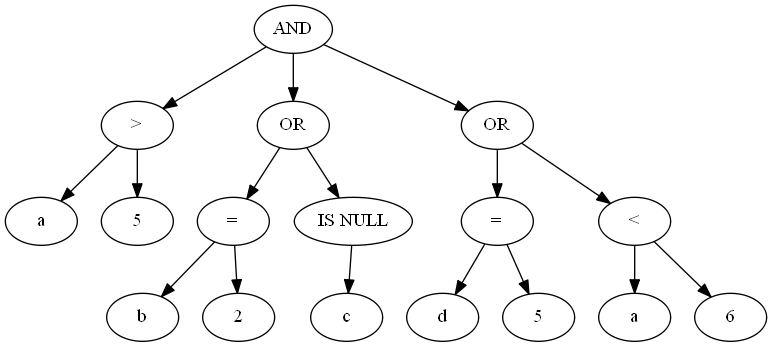
\includegraphics[scale=0.6]{Bilder/sort_ex0.png}
\caption{Sortierbeispiel: Ausgangsbaum}
\label{fig:sort_ex0}
\end{figure}

Wir bemerken, dass wir einen kommutativen Operator (AND) als Wurzelknoten haben und sortieren daher die unmittelbaren Kinder von AND, also \verb|{>,OR,OR}| zu \verb|{OR,OR,>}|, wie in Abbildung \ref{fig:sort_ex1} zu sehen ist.

\begin{figure}
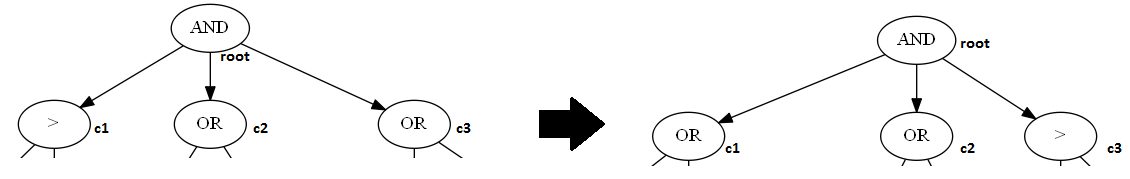
\includegraphics[scale=0.55]{Bilder/sort_ex12.png}
\caption{Sortierbeispiel: Sortierung der ersten Ebene}
\label{fig:sort_ex1}
\end{figure}

Wir fahren dann fort und führen sortieren rekursiv auf den Kindknoten $c_1,c_2$ und $c_3$ auf. Am Ende erhalten wir den Ausdruck \verb| (b=2 OR c IS NULL) AND (a<6 OR d=5) AND a<5|, welcher durch den Baum in Abbildung \ref{fig:sort_exfin1} dargestellt wird.

\begin{figure}
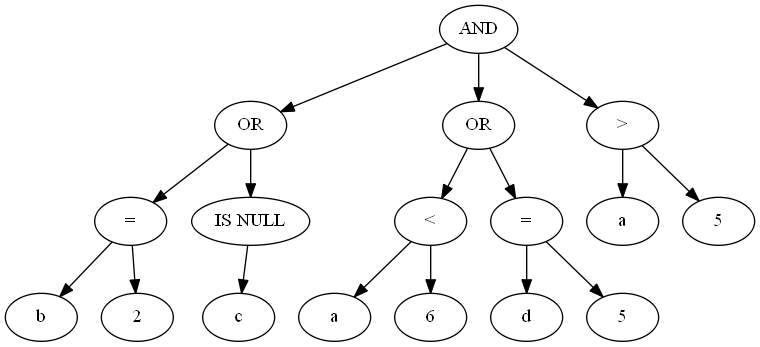
\includegraphics[scale=0.55]{Bilder/sort_exfin1.png}
\caption{Sortierbeispiel: Vorläufiges Ende des Sortierens}
\label{fig:sort_exfin1}
\end{figure}

Wenn wir uns Abbildung \ref{fig:sort_exfin1} genauer betrachten, so fällt auf, dass keine eindeutige Ordnung zugrunde liegt. Die beiden Bäume $T(c_1)$ und $T(c_2)$ repräsentieren beide den Operator \verb|OR|. Es ist mit den bisherigen Regeln nicht klar, was passiert, wenn zwei Geschwisterknoten, den gleichen Operator repräsentieren.

Haben wir also den Fall, dass zwei Kindknoten $c_i,c_j$ von $T(r)$ den gleichen Operator repräsentieren müssen wir rekursiv die beiden Teilbäume $T(c_i)$ und $T(c_j)$ untersuchen. Wir begehen dabei eine gleichzeitge und schrittweise Tiefensuche in beiden Bäumen durch, in dem wir sukzessive einen Schritt einer Tiefensuche in einem Baum, dann im anderen Baum durchführen und schließlich einen nächsten Schritt, in gleicher Weise durchführen. Wir bezeichen die Knoten, bei denen sich die Tiefensuche in einem aktuellen Moment befindet als $v_i\in T(c_i)$ und $v_j\in T(c_j)$. Sobald in einem Schritt $v_i \neq v_j$ ist, entscheiden wir anhand von $\mathit{order}(v_i)$ und $\mathit{order}(v_j)$, welcher Teilbaum vor dem anderen erscheinen soll. $T(c_i)$ erscheint damit vor $T(c_j)$, wenn $\mathit{order}(v_i) < \mathit{order}(v_j)$. Dabei schließen wir Blattknoten von der Betrachtung aus. Trifft die Tiefensuche also in einem Schritt auf beiden Seiten auf Blattknoten, so werden diese nicht mit einbezogen.

Ist die Tiefensuche beendet und es gab zu keine Zeitpunkt zwei innere Knoten in beiden Bäumen mit unterschiedlichen Operatoren, so sind offensichtlich die beiden Teilbäume $T(c_i)$ und $T(c_j)$ strukturell gleich, sie haben also identische innere Knoten. In diesem Fall unterscheiden sich beide Bäume nur durch ihre Blattknoten. Wir bezeichnen die Blattknoten von $T(c_i)$ mit $leaf(c_i)$ und in entsprechender Weise $leaf(c_j)$ die Blattknoten von $T(c_j)$. Wir sortieren diese Blattknotenmengen jetzt lexikographisch. Es ist offensichtlich, dass beide Blattknotenmengen gleich mächtig sind, da ansonsten bereits ein Unterscheid beim Tiefensuchvergleich aufgefallen wäre. Wir gehen jetzt sukzessive beide, sortieren Blattknotenmengen durch und vergleichen jeweils das $i.$ Element dieser Mengen, wobei $1\le i \le n$, mit $n=\vert \mathit{leaf}(c_i)\vert = \vert \mathit{leaf}(c_j) \vert$. Unterscheiden sich die $i.$ Elemente der zwei Mengen, dann erscheint $T(c_i)$ vor $T(c_j)$, wenn das i. Element in $\mathit{leaf(c_i)}$ lexikographisch kleiner ist als das i. Element in $\mathit{leaf(c_j)}$.

Zu beachten ist, dass wenn innerhalb eines Teilbaumes $T(c_i)$ wieder die Situation eintritt, dass es zwei Kinder $d_i,d_j\in\mathit{children}(c_i)$ gibt, mit $d_i=d_j$, aber $i\neq j$, dann wird dieser Fall zuerst behandelt. Wir behandeln also Kinder mit gleichen repräsentierten Operatoren von den Blättern aus, also Bottom-Up.

Als Beispiel betrachten wir den Baum in Abbildung \ref{fig:sort_exfinb0}.

\begin{figure}
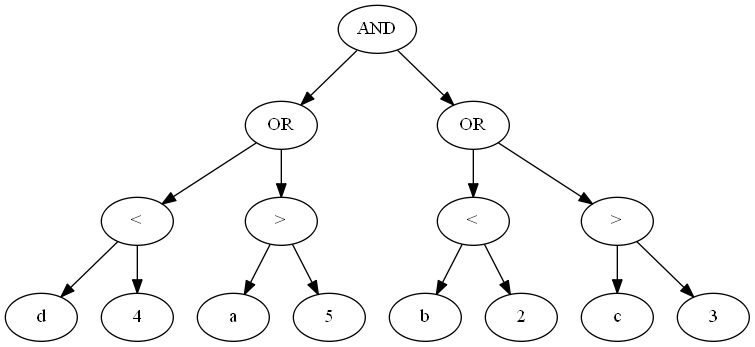
\includegraphics[scale=0.55]{Bilder/sort_exfinb0.png}
\caption{Sortierbeispiel: strukturell identische Teilbäume}
\label{fig:sort_exfinb0}
\end{figure}

Wie wir sehen, sind alle inneren Knoten gleich. Es unterscheiden sich nur die Blattknoten, weshalb eine simultane Tiefensuche über $T(c_1)$ und $T(c_2)$ keine Unterschiede aufgezeigt hat. Die Menge der Blattknoten sind $\mathit{leaf}(c_1) = \{d,4,a,5\}$ und $\mathit{leaf}(c_2) = \{b,2,c,3\}$. Wir sortieren diese Mengen nun und erhalten: $\mathit{leaf'}(c_1) = \{4,5,a,d\}$ und $\mathit{leaf'}(c_2) = \{2,3,b,c\}$.
Wir gehen nun sukzessive beide Mengen durch und vergleichen zunächst das 1. Element beider Mengen. Diese beiden ersten Elemente unterscheiden sich bereits und weil $4 > 2$ müssen die beiden Bäume $T(c_1)$ und $T(c_2)$ vertauscht werden. Wir erhalten also den finalen, sortierten Baum, der in Abbildung \ref{fig:sort_exfinb1} zu sehen ist.

\begin{figure}
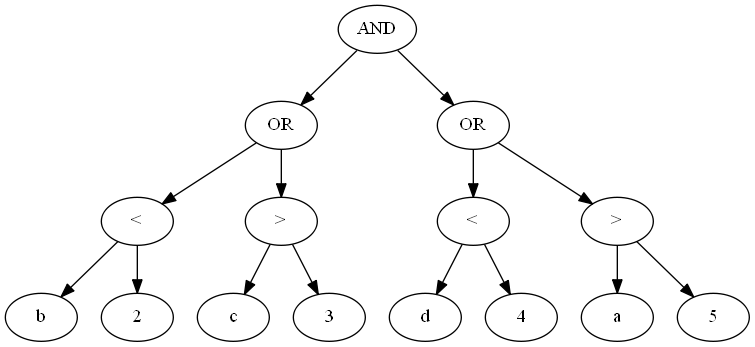
\includegraphics[scale=0.55]{Bilder/sort_exfinb1.png}
\caption{Sortierbeispiel: umsortierte Teilbäume}
\label{fig:sort_exfinb1}
\end{figure}



\subsection{GROUP BY / HAVING}

Bisher haben wir den SELECT-, FROM- und WHERE-Teil einer SQL-Anfrage bearbeitet und betrachtet. Anfragen, die einen GROUP BY-Teil enthalten müssen auch nach festen Regeln angepasst werden. Da die Reihenfolge innerhalb dieses Teils unwichtig ist, sortieren wir die Spaltennamen lexikographisch. Diese sind bereits automatisch benannt nach dem Schema \verb|aN| mit $N\in \{1,2,...\}$ (siehe Unterabschnitt \ref{subsec:from}). Demzufolge erscheinen zuerst Tabellennamen und dann Aggregationsfunktionen.

Der HAVING-Teil wiederum ähnelt von seiner Struktur dem WHERE-Teil. Es handelt sich ebenso um einen komplexeren Ausdruck. Wir behandeln daher den HAVING-Teil so, wie den WHERE-Teil im Unterabschnitt \ref{subsec:where}.

Nicht wichtig für die einheitliche Anpassung ist, ob die Tabellen bzw. Aggregationsfunktionen im GROUP BY-Teil auch im SELECT-Teil vorkommen. Dies könnte aber auf einen ungewollten Fehler des Lernenden hinweisen. Diese Information wird daher im Preprocessing (siehe Abschnitt \ref{subsec:preprocess}) mit aufgenommen. 

\subsection{ORDER BY}

Der ORDER BY-Teil kann nicht im Sinne der Standardisierung angepasst werden. Die hier angegebene Reihenfolge kann nicht verändert werden ohne den Sinn des Ausdruckes zu ändern. Die Anpassung beschränkt sich also auf das Umbenennen der Tupelvariablen, wie es im Unterabschnitt \ref{subsec:from} beschrieben ist.

Interessant für das Preprocessing sind allerdings andere Informationen über ORDER-BY. So merken wir uns, ob die Anfrage ORDER BY-Klauseln mit einem expliziten ASC enthält, da dies unnötig ist.

\subsection{Abschluss}

Wir fassen die einzelnen Schritte noch einmal kurz zusammen: Zunächst haben wir den \verb|FROM|-Teil der Anfrage vereinheitlicht, indem wir einheitliche Tupelvariablen erzeugt haben, nachdem alle Tabellen im \verb|FROM|-Teil lexikographisch sortiert wurden. Alle neu erzeugten Variablennamen wurden im Rest der Anfrage korrekt eingesetzt bzw. ersetzt. Finden wir in diesem Schritt im \verb|FROM|-Teil bereits zwei gleiche Tabellen mit unterschiedlichen Aliasen, so könnte ein Selbstverbund dadurch entstehen. Um mehrdeutigen zu vermeiden, erzeugen wir eine Kopie der vorliegenden Anfrage und vertauschen die gleichen Tabellennamen im \verb|FROM|-Teil. Wir erhalten somit für jeden Selbstverbund einen zusätzlich zu untersuchenden Baum. Am Ende prüfen wir ob einer dieser Bäume syntaktisch äquivalent ist mit einem der erzeugen Bäumde, der zweiten Anfrage. Danach haben wir den \verb|WHERE|-Teil bearbeitet. Wir haben zunächst unnötige Klammern entfernt und die Formeln in die KNF überführt. Danach haben wir einfache syntaktische Varianten ersetzt um eine einheitlichere Darstellung zu erhalten. Dazu gehörte es auch Unteranfragen aufzulösen oder, wenn nicht möglich, in eine \verb|EXISTS|-Unteranfrage zu überführen. Anschließend haben wir innere Verbunde (JOINs), die im \verb|FROM|-Teil formuliert wurden, in den \verb|WHERE|-Teil überführt. Eine der letzten Schritte war das Behandeln der Vielfalt der Operatoren. Hier haben wir für alle nicht-kommutativen Operatoren ihre alternativen Schreibweisen konjunktiv-verknüpft mit in die Formel aufgenommen. Nach diesem Schritt müssen wir nun die KNF wiederherstellen, da diese durch hinzufügen von \verb|AND|-Knoten zerstört sein kann. Schlussendlich haben wir den gesamten \verb|WHERE|-Teil sortiert, um eine Vereinheitlichung zu erreichen.

\section{Weitere Betrachtungen}

\subsection{JOINS}

Wir betrachten in diesem Abschnitt die Behandlung von JOINs. Wir untersuchen wie wir die unterschiedlichen Verbundstypen vereinfachen oder in eine einheitliche Form umwandeln können. Weiterhin interessiert uns die Frage, wie wir unnötige JOINs erkennen können. Wir diskutieren in wie weit eine automatische Entfernung von unnötigen JOINs Sinn macht und wie das Feedback für den Lernenden aussehen kann.

Vorab möchten wir bemerken, dass die Standardisierung und Eliminierung von JOINs eine fortgeschrittene Strategie darstellt. Diese wird daher nicht im Prototypen auftauchen. Dennoch betrachten wir die theretischen Grundlagen ausreichend und tiefgründig, so dass eine Implementation leicht möglich sein wird.

\subsubsection*{CROSS JOIN}

Ein \verb|CROSS JOIN| zweier Relationen liefert das kartesische Produkt beider zurück. Das Schlüsselwort \verb|CROSS JOIN| unter \verb|FROM| markiert diesen. Das Schlüsselwort kann allerdings auch weggelassen und durch ein Komma ersetzt werden. Um eine einheitliche Darstellung dieses Verbundtypes zu gewährleisten, werden wir das Schlüsselwort \verb|CROSS JOIN| ersetzen, so dass wir eine Liste von Tabellen unter \verb|FROM| erhalten, welche mit Komma getrennt sind.

\subsubsection*{NATURAL JOIN}

Ein natürlicher Verbund (NV) ist ein Verbund im \verb|FROM|-Teil. Er wird markiert durch die Schlüsselworte \verb|NATURAL JOIN ON|. Der Verbund zweier Relationen erfolgt über die Attribute, die in beiden Relationen die gleiche Bezeichnung haben. Gibt es keine solchen Attribute, ist das Ergebnis das kartesische Produkt beider Relationen.

Es gibt zwei Möglichkeiten natürliche Verbunde zu standardisieren. Die erste Möglichkeit besteht darin,   alle Verbundskriterien zu durchsuchen. Stellt man fest, dass die Attribute bei einem Verbundskriterium identisch sind, so handelt es sich um einen natürlichen Verbund. Man könnte diese Kriterien nun streichen und mit dem Schlüsselwort \verb|NATURAL JOIN| explizit kennzeichnen, dass es sich um einen NV handelt. Bei dieser Möglichkeit können aber Probleme auftreten. Angenommen der Lernende L reicht eine Lösung ein, die einen natürliche Verbund zwischen \verb|t1| und \verb|t2| explizit enthält. Weiterhin gibt es kein namensgleiches Attribut in \verb|t1| und \verb|t2|, so dass der natürliche Verbund im Prinzip ein kartesisches Produkt ist. In der Musterlösung stehen \verb|t1| und \verb|t2| nur unter \verb|FROM| um eben dieses Produkt zu erzeugen. Die Methode 1 würde nun garkeine Anpassung machen, da es kein Kriterium für einen potentiellen natürlichen Verbund in der Anfrage des L findet. Als Folge können wir die beiden Anfragen nicht matchen, obwohl beide das gleiche tun.

Die zweite Möglichkeit besteht darin explizite natürliche Verbunde umzuschreiben, in dem wir das Schlüsselwort \verb|NATURAL JOIN| entfernen und beide Relationen durchsuchen nach gleichnamigen Attributen. Haben wir solche gefunden, so fügen wir diese explizit als Verbundskriterien ein. Haben wir keine solche Kriterien gefunden, handelt es sich um ein kartesisches Produkt. Wir fügen in diesem Fall die zweite Tabelle unter \verb|FROM| hinzu und eliminieren das Schlüsselwort \verb|NATURAL JOIN|.

Beide Methoden haben einen gewissen Aufwand zu bewältigen. Bei Methode 1 müssen wir alle Verbundskriterien durchsuchen, was im schlimmsten Fall alle atomaren Formeln im \verb|WHERE|-Teil sein können. In Methode 2 müssen wir zwei Relationen paarweise nach gleichnamigen Attributen durchsuchen.
Wir entscheiden uns für die 2. Methode, da Methode 1, wie oben erwähnt, Schwächen bei der Umwandlung hat. Weil wir den \verb|NATURAL JOIN| unter \verb|FROM| also auflösen, schreiben wir diesen gleich als \verb|INNER JOIN| unter die \verb|WHERE|-Bedingung, wie das  Beispiel \ref{bsp:natjoin} zeigt (angenommen \textit{table1} und \textit{table2} haben beide eine gleichnamige Spalte namens \textit{id}).

Die eben aufgeführten Transformationen sind nur möglich, wenn der \verb|SELECT|-Teil nicht aus der Wildcard \verb|*| besteht. Bei einem NV wird in einem solchen Fall die Spalte mit dem gleichnamigen Attribut in der zweiten Tabelle eliminiert. Bei einem Verbund mit expliziter Angabe des Verbundskriterium wird dies nicht realisiert. Deswegen sind natürliche Verbunde, die im \verb|SELECT|-Teil die Wildcard \verb|*| enthalten, nicht in explizite Verbunde unter \verb|WHERE| überführbar.

\begin{figure}
\begin{verbatim}
Vorher:
SELECT t1.col1 FROM table1 t1 NATURAL JOIN table2 t2

Danach:
SELECT t1.col1 FROM table1 t1, table2 t2 WHERE t1.id=t2.id
\end{verbatim}
\caption{Beispiel: Standardisierung eines natürlichen Verbundes}
\label{bsp:natjoin}
\end{figure}

\subsubsection*{OUTER JOIN}

Bei einem \verb|OUTER JOIN| unterscheiden wir zwischen einem \verb|LEFT OUTER JOIN| und einem \verb|RIGHT OUTER JOIN|. Ein \verb|FULL OUTER JOIN| ist die Verbindung, also ein \verb|UNION| vom linken und rechten \verb|OUTER JOIN|. Wir betrachten daher exemplarisch zunächst den \verb|LEFT OUTER JOIN|, da sich die Betrachtungen dann äquivalent auf den rechten Verbund und damit auf den \verb|FULL OUTER JOIN| übertragen lassen.

Zunächst ist zu klären, wie der \verb|OUTER JOIN| alternativ formuliert werden kann. Dazu gehen wir kurz darauf ein, was ein \verb|LEFT OUTER JOIN| genau macht. Die ``linke'' Tabelle wird vollständig aufgeführt. Dann wird jeder Eintrag der Tabelle sukzessive betrachtet. Gibt es im aktuellen Eintrag einen Verbundspartner in der ``rechten'' Tabelle (vorgegeben durch das Verbundskriterium), dann werden die Daten der ``rechten'' Tabelle an den Eintrag angehangen. Ist dies nicht der Fall, wird der Eintrag mit \textit{NULL} Einträgen aufgefüllt. 

Um die Umwandlung eines \verb|LEFT OUTER JOIN| zu demonstrieren, betrachten wir folgendes Beispiel:

\begin{figure}[h]
\begin{verbatim}
SELECT e.empno, e.job, d.dname 
FROM dept d 
LEFT JOIN emp e ON e.deptno = d.deptno 
WHERE e.sal > 2000
ORDER BY e.empno
\end{verbatim}
\caption{OUTER JOIN Beispiel}
\end{figure}

Wir haben also zwei verschiedene Mengen von Einträgen. Zum einen Einträge, die einen Verbundspartner besitzen und Einträge, die keinen solchen Partner haben. Anbieten würde sich an dieser Stelle die Verwendung einer Vereinigung (\verb|UNION|) der beiden, eben genannten Mengen. Dabei ist die Umwandlung in ein solches Statement mit einem \verb|UNION| keinesfalls trivial und unterliegt einigen Einschränkungen. 

Ziel ist es also zwei SQL-Anfragen zu formulieren, die jeweils für die oben genannten Mengen stehen. Anschließend werden diese Mengen mit einem \verb|UNION| verbunden.

Für die SQL-Anfrage, welche die Menge der Verbundspartner angibt, übernehmen wir zunächst den \verb|SELECT|-Teil. Die zwei Tabellen, die am Verbund beteiligt sind werden im \verb|FROM|-Teil nun als \verb|CROSS JOIN| aufgeschrieben, also mit Komma getrennt. Der \verb|WHERE|-Teil wird ebenfalls vom gegebenen \verb|OUTER JOIN|-Statement übernommen und durch die Angabe des Verbundskriteriums ergänzt.
Wir erhalten also die folgende Anfrage bezüglich unseres Beispiels:

\begin{figure}[h]
\begin{verbatim}
SELECT e.empno, e.job, d.dname 
FROM dept d, emp e
WHERE d.deptno = e.deptno
AND e.sal > 2000
ORDER BY e.empno
\end{verbatim}
\caption{OUTER JOIN Umwandlung, 1. Teil}
\end{figure}

Nun muss noch die Teilmenge aller Tupel hinzugefügt werden, die keinen Verbundspartner haben. Wir übernehmen zunächst wieder den \verb|SELECT|-Teil der Ursprungsanfrage, ersetzen aber alle Spaltennamen der ``rechten'' Tabelle mit \verb|NULL|, weil diese Werte aufgrund fehlender Verbundspartner nicht belegt sind. Diese Ersetzungen müssen ebenso im \verb|WHERE|-Teil stattfinden. Die rechte Tablle wird aus dem \verb|FROM|-Teil gestrichen. Nun passen wir den \verb|WHERE|-Teil an. Hier könnte man auf die Idee kommen mit einem \verb|NOT IN| Semijoin zu prüfen, dass auch nur Tupel ohne Verbundspartner aufgenommen werden. Erlaubt  das Verbundskriterium in der ``linken'' Tabelle \verb|NULL|-Werte, so würden diese Einträge nicht erscheinen. Bei einem \verb|LEFT OUTER JOIN| sind diese Tupel aber mit erfasst. Es bietet sich daher eine \verb|NOT EXISTS|-Unterabfrage an. 

\begin{figure}[h]
\begin{verbatim}
SELECT NULL, NULL, d.dname
FROM dept d 
WHERE NOT EXISTS(
    SELECT 1 FROM emp e WHERE d.deptno = e.deptno )
AND NULL > 2000
ORDER BY e.empno
\end{verbatim}
\caption{OUTER JOIN Umwandlung, 2. Teil}
\end{figure}

Nun müssen beide Anfragen mit einem \verb|UNION ALL| verknüpft werden. Dabei können wir das \verb|ORDER BY|-Statement ausklammern, da dieses erst auf dem Datensatz, der mit \verb|UNION ALL| erzeugt wurde, ausgeführt wird. Unser Endergebnis bezogen auf unser Beispiel lautet also:

\begin{figure}[h]
\begin{verbatim}
SELECT e.empno, e.job, d.dname FROM dept d, emp e
WHERE d.deptno = e.deptno AND e.sal > 2000
    UNION ALL
SELECT NULL,NULL,d.dname FROM dept d 
WHERE NOT EXISTS(
  SELECT 1 from emp e where d.deptno = e.deptno)
AND NULL > 2000
ORDER BY empno
\end{verbatim}
\caption{OUTER JOIN Umwandlung, finaler Schritt}
\end{figure}

Wie man bereits am Beispiel sieht, könnte man im \verb|WHERE|-Teil den Ausdruck \verb|NULL > 2000| zu \verb|NULL| vereinfachen oder gar die zweite Anfrage komplett streichen, da sie nie erfüllt ist. 

Eine Besonderheit stellt das \verb|GROUP BY|-Statement dar. Dies wurde nicht im Beispiel benutzt, daher betrachten wir nun im Folgenden, wie damit zu verfahren ist.

Wird in der \verb|OUTER JOIN| Abfrage nach mindestens einem Attribut der ``rechten'' Tabelle gruppiert, so müssen wir die Gruppierung in eine weitere Anfrage schachteln. Dazu bauen wir die Anfrage, wie oben beschrieben, auf und streichen das \verb|GROUP BY|-Statement zunächst. Aggregationsfunktion \textit{agg(x)} werden ersetzt zu \textit{x}. Um die dann entstandene, mit \verb|UNION ALL| verknüpfte SQL-Anfrage A schachteln wir eine weitere Anfrage B. Der \verb|SELECT|-Teil von B entspricht dem, der ursprünglichen \verb|OUTER JOIN|-Anfrage. Der \verb|FROM|-Teil von B entspricht der konstruierten Anfrage A. Einen \verb|WHERE|-Teil von B gibt es nicht, da dieser bereits in der Anfrage A eingearbeitet wurde. Ergänzt wird die Anfrage B mit dem \verb|GROUP BY|- und \verb|ORDER BY|-Statement der Ursprungsanfrage.

Existiert im \verb|GROUP BY|-Teil der Originalanfrage kein Attribut der ``rechten'' Tabelle, ist die eben genannte Schachtelung nicht notwendig. Es reicht hier aus den \verb|GROUP BY|-Teil einfach in die Konstruierten Teilanfragen mit einzubeziehen. Grund dafür ist, dass wir disjunktive Gruppierungen in beiden Anfragen erhalten und diese ohne Probleme mit \verb|UNION ALL| vereinigen können.

Dies waren alle notwendigen Schritte um einen \verb|LEFT OUTER JOIN| äquivalent in eine komplexe Anfrage mit \verb|UNION ALL| und Semijoins zu überführen. Zu Bemerken ist an dieser Stelle, dass ein \verb|RIGHT OUTER JOIN| entsprechend behandelt wird, nur mit umgekehrten Seiten. Einen \verb|FULL OUTER JOIN| erhalten wir durch ein \verb|UNION| vom \verb|LEFT OUTER| und \verb|RIGHT OUTER JOIN|. 

Nach dieser Betrachtung müssen wir jedoch feststellen, dass die Umwandlung eines \verb|OUTER JOIN| recht vielschichtig und aufwendig ist. Es ist zwar möglich diesen äquivalent umzuformen, allerdings wird der Ausdruck dadurch enorm aufgebläht. Weiterhin funktioniert diese Umwandlung nur in eine Richtung problemlos, nämlich vom \verb|JOIN| zum \verb|UNION|-Ausdruck. Umgekehr ist es sehr aufwendig festzustellen, ob ein \verb|UNION ALL| auch ein \verb|OUTER JOIN| ist, da man zum Beispiel Vergleiche mit \verb|NULL|-Werten (wie im Beispiel: \verb|NULL > 2000|) gewöhnlich nicht ausschreibt oder gar entfernt. Unser Programm soll \verb|OUTER JOIN| daher nicht in einen \verb|UNION ALL| Ausdruck umwandeln. Wir beschränken uns in der Praxis also darauf, einen \verb|OUTER JOIN| unter \verb|FROM| rein syntaktisch zu erkennen und nicht umzuwandeln.

\subsubsection*{INNER JOIN}

Unter einem \verb|INNER JOIN| verstehen wir den Verbund zweier Tabellen unter \verb|FROM|, mit den Schlüsselworten \verb|INNER JOIN|. Ein solcher Verbund kann leicht als \verb|CROSS JOIN| mit Auswahl in der \verb|WHERE|-Bedingung formuliert werden. Dazu entfernen wir den \verb|INNER JOIN| aus dem \verb|FROM|-Teil und erzeugen einen \verb|CROSS JOIN|. Die Verbundbedingungen werden unter \verb|WHERE| eingefügt.

Ein explizit aufgeschriebener \verb|INNER JOIN| kann auch ein \verb|NATURAL JOIN| sein. Da wir solche Verbunde aber auch als \verb|CROSS JOIN| aufschreiben wollen (siehe oben), müssen wir diesen Spezialfall nicht gesondert betrachten. Das folgende Beispiel soll die Umwandlung von \verb|INNER JOIN| verdeutlichen:

\begin{figure}[h]
Eingabe:\\
\verb|SELECT * FROM emp e INNER JOIN dept d ON e.deptno.id = d.deptno|\\

Umwandlung:\\
\verb|SELECT * FROM emp e, dept d WHERE e.deptno = d.deptno|\\
\caption{Umwandlung von INNER-JOIN}
\end{figure}


\subsubsection{JOIN-Eliminierung}

Im vorherigem Abschnitt haben wir bereits alle üblichen Verbunde betrachtet und gezeigt, wie wir diese äquivalent umformen können. Wir haben erreicht, dass alle Verbunde unter \verb|FROM| ersetzt wurden zu \verb|CROSS JOIN| mit Auswahlkriterien unter \verb|WHERE|. Wir möchten daher in diesem Abschnitt klären, welche Möglichkeiten es gibt, die so entstandenen Verbunde, zu eliminieren, wenn sich herausstellt, dass sie überflüssig sind.

Wenn nur Schlüsselattribute einer Tupelvariable X benutzt werden und diese mit \hyphenation{Fremd-schlüs-sel-at-tri-but-en} einer anderen Tupelvariable Y verglichen werden, dann ist X überflüssig.

Ziel dieses Abschnittes ist es, eine Idee vorzustellen, wie redundante Verbunde mit Hilfe von referentiellen Integritätsbedingungen (RI) gefunden werden können. 
Die mögliche Anwendung ist natürlicherweise die Entfernung einer Relation bei dem der Verbund aus Tabellen besteht, die durch eine RI-Bedingung verbunden ist (nachfolgend als RI-Joins bezeichnet) und bei der die Tabelle, die den Primärschlüssel enthält nur im Join referenziert wird. Ein RI-Join besteht natürlicherweise aus einem Primärschlüssel- und einem Fremdschlüsselattribut.

Das Verfahren wird in der Arbeit \cite{joinelem2} näher vorgestellt und läuft im wesentlichen in 4 Schritten ab.

\begin{enumerate}
\item Wir bilden zunächst transitive Spaltenäquivalenzklassen von allen Joinprädikaten. Ist als \verb|A=B| und \verb|B=C|, dann können wir transitiv ableiten, dass ebenso \verb|A=C| gilt. Alle drei Spalten, \verb|A,B,C| befinden sich dann in einer Äquivalenzklasse.

\item Alle Tabellen unter \verb|FROM|, die mit RI-Joins verknüpft sind, werden in zwei Gruppen eingeteilt. Tabellen in der R-Gruppe sind entfernbar (removable) und Tabellen in der N-Gruppe sind nicht entfernbar (non-removable). Die notwendige Bedingung, die bestimmt, wann eine Tabelle in die R-Gruppe gehört ist, dass es eine parent-table für irgendeine RI. Dies ist jedoch nicht die einzige notwendige Bedingung. Andere, zu erfüllende Bedingung, sind weitaus komplexer und sind für die Präsentation des Ansatzes dieser Methode zu umfangreich. Nachzulesen ist das detaillierte Verfahren in der Arbeit \cite{joinelem2}.

\item Alle Tabellen in der R-Gruppe werden entfernt.

\item Da es Fremdschlüssel geben kann, die \verb|NULL|-Werte erlauben, ist es notwendig, ein \verb|IS NOT NULL|-Prädikat dort hinzuzufügen, wo die parents einer RI entfernt wurden und \verb|NULL|-Werte erlaubt sind.
\end{enumerate}

Als visuelles Hilfsmittel verwendet das Verfahren sogenannte Joingraphen $G=(V,E)$. Die Knotenmenge $V$ besteht aus Joinattributen. Eine Kante zwischen zwei Knoten $u,v$ existiert genau dann, wenn $u$ und $v$ Teil eines Joinprädikates sind. Handelt es sich bei dem Join um einen RI-Join, also ein Primär-/ Fremdschlüssel Join, dann sind $u,v$ durch eine gerichtete Kante verbunden, wobei der Pfeil dann vom Fremdschlüsselattribut/Kind zum Primärschlüsselattribut/Eltern geht.

Nimmt man sich diese Joingraphen zur Hilfe gibt es drei auszuführende Schritte. Im ersten Schritt wird der Joingraph erzeugt, nach oben genannten Regeln. Dabei werden RI-Joins noch nicht gerichtet dargestellt. Wir erhalten $G_1$.

Im zweiten Schritt fügt man alle transitiv-implizierten Joins als nicht RI-Joins hinzu und markiert die echten RI-Joins entsprechend mit Pfeilen. Wir erhalten $G_2=(V_2,E_2)$

Im dritten Schritt werden unnötige (redundante) Joins entfernt. Ein Knoten $v\in V_2$ ist entfernbar, wenn $v$ Teil eines RI-Joins ist und $v$ nur als Joinkriterium in der Anfrage vorkommt, also weder im \verb|SELECT-, WHERE-| oder \verb|GROUP BY-|Statement vorkommt. Wir erhalten $G_3$, aus dem wir auch ablesen können welche Joins noch notwendig sind. 

Folgendes Beispiel soll das eben Erwähnte verdeutlichen.

\begin{lstlisting}[mathescape]
SELECT ps.partkey, avg(ps.supplycost)
FROM   supplier s, partsupp ps, customer c, orders o
WHERE  s.suppkey = ps.suppkey 
AND    s.suppkey = c.custkey
AND    c.custkey = o_custkey
AND    o.totalprice >= 100
GROUP BY ps.partkey
\end{lstlisting}

Wir erzeugen zunächst den ersten Joingraphen $G_1$, in dem wir jede Joinbedingug als verbundes Paar in den Graphen einfügen:

\begin{figure}[h]
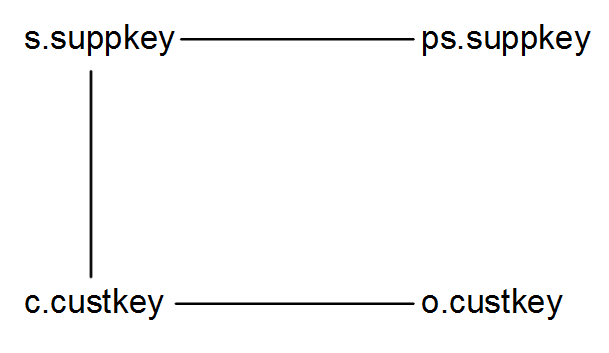
\includegraphics[scale=0.4]{Bilder/joinelem_g1.png}
\caption{$G_1$}
\end{figure}

Im zweiten Schritt fügen wir nun alle transitiv-implizierten Joins als nicht RI-Joins hinzu, also als ungerichtete Kanten. Wir weisen dann die RI-Joins aus, in dem wir sie als gerichtete Kanten markieren und erhalten damit $G_2$:

\begin{figure}[h]
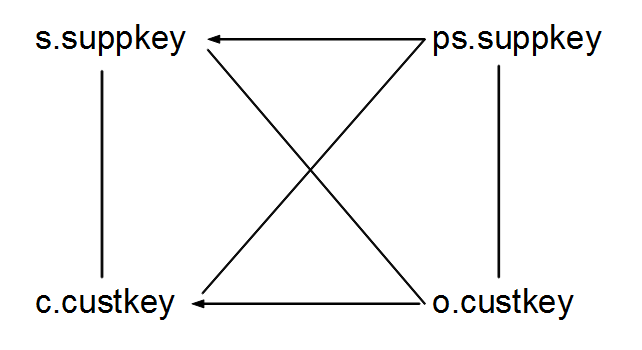
\includegraphics[scale=0.4]{Bilder/joinelem_g2.png}
\caption{$G_2$}
\end{figure}

Im letzten Schritt gehen wir alle Knoten sukzessive durch. Da jeder Knoten ein Attribut repräsentiert, prüfen wir ob das repräsentierte Attribut in einem Nicht-Join Prädikat unter \verb|WHERE|, im \verb|GROUP BY|- oder im \verb|SELECT|-Teil vorkommt. Ist dies nicht der Fall, eliminieren wir den Knoten und alle zugehörigen Kanten. In unserem Beispiel kommt weder \verb|s.suppkey| noch \verb|c.custkey| in den genannten Teilen der Anfrage vor. Wir löschen diese Attribute aus $G_2$ und erhalten $G_3$ mit nur noch einem, notwendigen Join:

\begin{figure}[h]
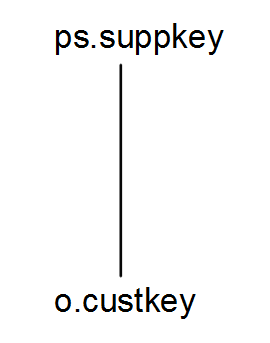
\includegraphics[scale=0.4]{Bilder/joinelem_g3.png}
\caption{$G_3$}
\end{figure}

Durch die Entfernung von Joinprädikaten kann es nun sein, dass auf einige Tabellen, die unter \verb|FROM| stehen, nicht mehr zugegriffen wird. Ist dies der Fall und sind weitere Bedingungen erfüllt, die detailliert in \cite{joinelem2} aufgeführt sind, so müssen diese Tabellen entfernt werden, da sonst ein ungewollter \verb|CROSS JOIN| entsteht, der u.a. zu vielen ungewollten Duplikaten führen kann.

Wir erhalten also folgende SQL-Anfrage:

\begin{lstlisting}[mathescape]
SELECT ps.partkey, avg(ps.supplycost)
FROM   partsupp ps, orders o
WHERE  o.custkey = ps.suppkey 
AND    o.totalprice >= 100
GROUP BY ps.partkey
\end{lstlisting}

Zu Bemerken ist, dass es noch mehr Fälle gibt, die der Algorithmus in \cite{joinelem2} behandelt. Der vorgestellte Ansatz entfernt nur eine Art von redundanten Joins. 

Redundante Joins zu finden ist keine triviale Aufgabe. Es gibt viele verschiedene Bedingungen die geprüft werden müssen und selbst dann gibt es keinen universellen Ansatz, der sämtliche redundante Joins entdeckt. Aufgrund dieser Komplexität, wird die Joineleminierung nicht in den Prototypen, der im Rahmen dieser Arbeit entsteht, Einzug halten. Für eine zukünftige Erweiterung des Programms um mehr semantic-checks, wäre dieser Ansatz aber gut geeignet.


\subsubsection*{OUTER JOIN-Eliminierung}

Innere Joins sind einfacher zu handhaben als äußere Joins. In der Arbeit \cite{outer2inner} wird ein Verfahren vorgestellt, welches \verb|OUTER JOIN| äquivalent in \verb|INNER JOIN| umwandelt. Das Verfahren ist komplex und mehrstufig, kann aber mit allen \verb|OUTER JOIN| umgehen. Der entstandene \verb|INNER JOIN| ist allerdings aufgebläht und nicht mehr lesbar, da er künstlich konstruiert ist. Im Rahmen unserer Arbeit interessiert dieser Fakt nur am Rande, im Zuge einer Erweiterung der semantischen Funktionen unseres Programmes, ist dieser Ansatz aber sicherlich erwähnenswert und interessant.

\section{Komplexität von SQL-Anfragen}

Durch Standardisierung zweier SQL-Abfragen \verb|query1| und \verb|query2| können wir durch einen syntaktischen Vergleich prüfen, ob es uns möglich war, beide gegeneinander zu matchen. Unabhängig vom Ergebnis dieses Matchings ist für den Lernenden wichtig, wie nah er an der Musterlösung dran war. Folgende Szenarien sind dabei denkbar. 

Im ersten Szenario konnte die SQL-Anfrage des Lernenden nicht mit der SQL-Anfrage der Musterlösung gematcht werden. Der Lernende benötigt nun ein Feedback um seine Fehler zu erkennen und um letztendlich einen neuen Lösungsvorschlag zu machen. 

In einem zweite Szenario konnte die SQL-Anfrage des Lernenden gematcht werden. Während des Standardisierungsprozesses seiner Anfrage, kann es aber sein, dass unnötige Klauseln entfernt wurden. In einem solchen Fall ist es von Interesse dem Lernenden mitzuteilen, dass seine Lösung noch nicht perfekt (im Sinne der Musterlösung) ist. 

Wir wollen im Folgenden nun Kriterien von Metainformationen festlegen. Diese Metainformationen der zwei Anfragen sollen dann jeweils miteinander verglichen werden. Finden wir bei einem solchen Vergleich Unstimmigkeiten in der Anzahl der jeweiligen Informationen, muss dies dem Lernenden mitgeteilt werden.

\subsection{Anzahl atomarer Formeln unter WHERE / Baumtiefe}

Die Studentenanfrage enthält vor der Transformation durch unser Programm mehr atomare Formeln als die Musterlösung, so wurden offensichtlich unnötige Formeln oder doppelte Formeln aufgeschrieben. Stellt unser Programm fest, dass beide Lösungen dennoch gleich sind, so muss dem Studenten mitgeteilt werden, dass er redundante Formeln eingebaut hat, welche die Lösung unnötig verkomplizieren. 

Gleichzeitig kann die unterschiedliche Tiefe des Parserbaumes der \verb|WHERE|-Klausel auch auf redundante Formeln hinweisen, die unser Programm durch Konstanten ersetzt hat, beispielsweise arithmetisch/logische Ausdrücke, die nur Konstanten als Operanden haben und damit bereits auswertbar sind.

\subsection{Anzahl benutzter Tabellen unter FROM}

Der Lernende könnte durch gewisse Semi-Joins unter \verb|WHERE| durchaus eine andere Anzahl an Tabellen im \verb|FROM|-Teil benutzten, als die Musterlösung. 

\subsection{Existenz von Teilen der SQL-Anfrage}

Geraden wenn der Lernende eine falsche Lösung einsendet, kann es sein, dass er sogar wichtige Teile einer Anfrage nicht benutzt, die aber von der Musterlösung verwendet wird. So ist es sinnvoll zu vergleichen, ob sowohl die Musterlösung, als auch die Lösung des Studenten einen nicht leeren \verb|SELECT-, FROM-, WHERE-, GROUP BY-| und \verb|ORDER BY-|Teil hat. Unterschiede müssen dem Lernenden mitgeteilt werden. Dabei ist sowohl die Information interessant, ob ein gewisser Teil existiert, als auch die Anzahl der Attribute oder Formeln im jeweiligen Teil der Anfrage.

\subsection{Anzahl von JOINs / Unterabfragen}

Sehr viele Fehler bei Anfängern finden sich im Bereich JOINs. Gerade deswegen ist es für den Lernenden interessant, ob er mehr oder weniger JOINs verwendet hat, als die Musterlösung. Im selben Atemzug sind Unterabfragen genannt, die entweder zu zaghaft oder zu häufig von Lernenden eingesetzt werden. Daher sollte auch diese Anzahl überwacht werden.

\subsection{Anzahl der Operatorkompressionen}

Wie im vorherigen Abschnitt bereits erklärt ist der ZQL-Parserbaum nicht binär. Dadurch kann es durch zu vorsichtige Klammersetzung passieren, dass ein Teilbaum mit zwei Ebenen entsteht, obwohl nur ein Operator beteiligt ist. Erklärt ist dies im Abschnitt >>Funktionsweise des Parsers<<. Die dort vorgestellte Operatorkompression ist ein Verfahren um unnötige Klammerungen zu entfernen. Ist die Gleichheit der Lösung des Studenten mit der Musterlösung durch unser Programm gezeigt, aber die Studentenlösung musste mehr Operatorkompressionen durchführen, so hat der Student unnötige Klammern gesetzt, welche die Lösung wiederum unnötig verkomplizieren. Dies muss ihm durch unser Programm mitgeteilt werden.

\subsection{unnötiges DISTINCT}

Eine interessante Frage ist, ob ein \verb|DISTINCT| wirklich notwendig ist. Dies ist natürlich wichtig für den Vergleich zweier SQL-Anfragen. In \cite{brass2} wurde im Rahmen des SQLLint-Projektes bereits in dem Prototypen ein Checker eingebaut, der prüft ob \verb|DISTINCT| wirklich notwendig ist. Aber auch im Rahmen dieser Arbeit ist es notwendig zu wissen, ob das \verb|DISTINCT| notwendig ist. 

Auf den ersten Blick reicht es aus zu prüfen, ob die Musterlösung ein \verb|DISTINCT| enthält. Ist dies der Fall, so muss die Lösung des Lernenden das offensichtlich auch enthalten. Allerdings setzt dieser Denkansatz voraus, dass die eingetragene Musterlösung stets perfekt ist. Um Fehler vorzubeugen ist es besser, alle Anfragen auf unnötige \verb|DISTINCT| zu prüfen. So kann dem Korrektor beim Eintragen der Musterlösung bereits angezeigt werden, dass sein angegebenes \verb|DISTINCT| unnötig ist oder ob ein \verb|DISTINCT| notwendig wäre um Duplikate zu eliminieren. Auch wenn man sich weg bewegt vom Modell der Musterlösung und dem Vergleich mit dem Lernenden, ist dieser Check durchaus wichtig. Im Folgenden stellen wir daher einen Algorithmus vor, der erkennt ob die Lösung Duplikate enthalten kann oder nicht.

Dabei muss angemerkt werden, dass der nachfolgende Algorithmus die hinreichende Bedingung für ein unnötiges \verb|DISTINCT| prüft. Das bedeutet, dass wenn der Algorithmus sagt >>ja, \verb|DISTINCT| ist unnötig<<, können wir sicher sein, dass es tatsächlich unnötig ist. Sagt der Algorithmus allerdings >>nein<< bedeutet dies, nicht notwendigerweise, dass das \verb|DISTINCT| wirklich unnötig ist. Gewisse Sachverhalte findet der Algorithmus nicht.

Der Algorithmus ist nicht in unserem Programm implementiert. Wir beschreibe ihn aber im Folgenden so, dass er in einer Überarbeitung ohne Probleme integriert werden könnte. Der Algorithmus müsste dann in jedem Fall nach der Umwandlung des \verb|WHERE|-Teils in die KNF erfolgen, da dies eine Voraussetzung für den Algorithmus ist.

\subsection{verbale Beschreibung}

Es sei $\mathcal{K}$ die Menge aller Attribute, die als Aausgabespalten unter \verb|SELECT| vorkommen.
Wir fügen im nächsten Schritt nun alle Attribute $A$ zu $\mathcal{K}$ hinzu, für die $A=c$ bzw. $c=A$ in der \verb|WHERE|-Bedingung auftaucht. Hierbei wird, wie bereits erwähnt, vorausgesetzt, dass die Bedingung eine Konjunktion ist. Weiterhin ist zu bemerken, dass Unterabfragen vom Algorithmus ignoriert werden.

Solange eine der folgenden Aktionen zu einer Veränderung unseres Zustands führt, machen wir Folgendes:
\begin{itemize}
\item Wir fügen zur Menge $\mathcal{K}$ Attribute $A$ hinzu, wenn $A=B$ Teil der \verb|WHERE|-Bedingung ist und $B\in \mathcal{K}$ gilt.
\item Enthält $\mathcal{K}$ einen Schlüssel einer Tupelvariable, so fügen wir alle Attribute dieser Variable hinzu.
\end{itemize}

Enthält $\mathcal{K}$ nun von jeder Tupelvariable unter \verb|FROM| einen Schlüssel, so ist das \verb|DISTINCT| sicher überflüssig. Haben wir ein \verb|GROUP BY|-Statement so prüfen wir anstelle dessen, ob alle \verb|GROUP BY|-Spalten in $\mathcal{K}$ enthalten sind.

\subsection{Algorithmus aus \cite{sql1folien}}

Es sei unsere SQL-Anfrage der Form:

\begin{lstlisting}[mathescape]
SELECT $t_1$, ..., $t_k$
FROM $R_1\ X_1$, ..., $R_n\ X_n$
WHERE $\varphi$
\end{lstlisting}

Es sei $X=\{X_1, ..., X_n\}$ die Menge aller Tupelvariablen. Es sei $G=\{G_1, ..., G_m\}$ die Menge aller \verb|GROUP BY| Spalten.

Die einzelnen Attribute $t_i$ haben die Form $t = X.k$. Dabei ist $X$ eine Tupelvariable und $k$ ein Attribut. Wir bezeichnen die Menge aller $t_i$ mit $\mathcal{K}=\{t_1,...,t_k\}$.

\begin{lstlisting}[mathescape]
$\mathcal{K}$ = $\mathcal{K}\ \cup$ {A}, wenn $A=c$ als Konjunktion in WHERE auftaucht
do 
  $\mathcal{K'}$ = $\mathcal{K}$
  $\mathcal{K'}$ = $\mathcal{K'}\ \cup$ A, wenn $A=B\in$ WHERE-Bedingung und $B\in\mathcal{K}$
  $\mathcal{K'}$ = $\mathcal{K'}\ \cup$ S mit $S=\{b\in X\}$, wenn $t\in \mathcal{K'}$ ein Schluessel ist und t=X.k
while ($\mathcal{K}\ \neq\ \mathcal{K'}$)

if not Anfrage hat GROUP BY Statement:
  foreach $x\in X$ do
    if not ($\exists k\in \mathcal{K'}$ mit $k$ ist Schluessel von $x$)
      break and return NO
    endif
  done

if Anfrage hat GROUP BY Statement:
  foreach $g\in G$ do
    if $g\notin \mathcal{K'}$
      break and return NO
    endif
  done

return YES
\end{lstlisting}


Beispiel:

mit EMP und DEPT

\section{Alternativer Ansatz: Elementare Transformationen}

Der nun vorgestellte Ansatz stellt eine Alternative zur >>Anpassung durch Standardisierung<< dar. Beide Ansätze haben ähnliche Ideen, sind jedoch in ihrer Umsetzung verschieden. Beim Ansatz der Standardisierung haben wir zunächst eine SQL-Anfrage genommen und standardisiert. Dies geschah völlig unabhängig zu der zu vergleichenden, zweiten SQL-Anfrage. Es wurden gewisse allgemeine Regeln aufgestellt und nach diesen wurde jede SQL-Anfrage behandelt und angepasst. Der eigentliche Vergleich geschah dann aufgrund eines Vergleichs der standardisierten Anfragen und dem Vergleich von Metadaten (Anzahl Joins, Anzahl atomarer Formeln, etc.). Ein Nachteil von diesem Ansatz ist, dass wir für jedes mögliche Konstrukt in der SQL-Anfrage auch Regeln im System haben, damit wir jene Konstrukte auch anpassen und standardisieren können. Außerdem findet der Vergleich erst im allerletzten Schritt statt.

Die >>Anpassung durch elementare Transformationen<< stellt einen intuitiven Ansatz vor. Wir versuchen hier per Backtracking konkret eine Lösung der anderen anzugleichen. Damit haben wir einen konkreten Unterschied zum bisherigen Ansatz. Wir vergleichen die Lösung direkt und umgehen die Vorverarbeitungen. Im Wesentlichen geben wir also ganz allgemeine Regeln an und in jedem Schritt versuchen wir durch Anwendung dieser Regeln die SQL-Anfrage so anzupassen, dass sie auf unsere zu vergleichende Anfrage passt.

\subsection{Backtracking}

[Dieser Abschnitt ist experimentell]

Für das Backtracking an sich bietet sich die Programmiersprache PROLOG an. Das liegt daran, dass unsere allgemeine Regeln einfach formuliert werden können und bereits den Großteil des Programms stellen. Außerdem benutzt PROLOG die SLD-Resolution, um logische Anfragen auswerten zu können und das ist bereits ein Backtracking. Da wir in unserer Arbeit allerdings die Programmiersprache JAVA gewählt haben, können wir nicht auf PROLOG zurückgreifen. Viel mehr müssen wir das Backtracking selbst implementieren. 

Wir operieren weiterhin auf Parserbäumen, die so entstehen wie im Abschnitt >>Funktionsweise des Parsers<< erklärt wird. Es seien unsere zwei zu vergleichenden SQL-Anfragen mit \textit{Query1} und \textit{Query2} gegeben. Die dazugehörenden Parserbäume bezeichnen wir mit \textit{RT(Query1)} und \textit{RT(Query2)}. Wir versuchen im Folgenden \textit{Query1} an \textit{Query2} anzupassen.

Um nicht zu viele Regeln definieren zu müssen, werden wir Teile der Vorverarbeitung des ersten Ansatzes wieder verwenden. Wir formen beide Anfragen zunächst in die konjunktive Normalform um. Danach gehen wir nach dem folgendem Prinzip vor.

Es sei $\mathit{comm} = \{+,*,AND,OR,=\}$, die Menge aller kommutativen Operatoren. Wir gehen den Vergleich zweier (Teil-)Bäume rekursiv an, das bedeutet unser Algorithmus erhält stets zwei (Teil-)Bäume in Form von zwei Wurzelknoten. Als Ergebnis gibt der Algorithmus dann an, ob diese zwei (Teil-)Bäume unifiziert werden konnten. Im Folgenden wird der Algorithmus textuell beschrieben. Ein detaillierter Pseudocode ist im Anhang unter Abschnitt \ref{sec:backtrack1} zu finden.


TODO Algorithmus in Worten beschreiben: 
Zum einen haben wir kommutative Operatoren wie \verb|{+,*,AND,OR,=}|. Möchten wir zwei (Teil-)Bäume vergleichen, die einen solchen Operator als Wurzelknoten haben, so müssen wir uns im klaren sein, dass der gesuchte Operand an beliebiger Stelle auftauchen kann. Wir werden einen solchen Vergleich so angehen, dass wir uns den ersten Operanden aus Teilbaum 1 nehmen. Ist dieser Operand ein Ausdruck mit Operator $o_1$, dann suchen wir im zweiten Teilbaum nach einem Operanden, welcher auch ein Ausdruck ist mit Operator $o_2$ mit $o_1=o_2$. Ist dies gelungen, so wird verglichen, ob die Teilbäume mit der Wurzel $o_1$ und $o_2$ gleich sind. Dies geschieht dann rekursiv. Ist dies erfolgreich, so streichen wir aus den Ursprungsbäumen die Teilbäume mit Wurzel $o_1$ und $o_2$ und fahren mit dem nächsten Operanden aus dem ersten Teilbaum fort.

Operatoren, die nicht kommutativ sind, sind meistens Vergleichsoperatoren wie \verb|<=, < , > ,>=|. Haben wir zwei Teilbäume mit einem solchen Operator, so ist der Vergleich sehr einfach, denn die jeweiligen Teilbäume unter den Operatoren müssen absolut identisch sein. Dies wird wieder mittels Rekursion geprüft.

Haben wir im ersten Baum einen Vergleichsoperator ausgewählt und können diesen im zweiten Baum nicht finden, so müssen wir auch nach dem umgedrehten Operator in Baum 2 suchen. Finden wir einen solchen, dann vergleichen wir die zugehörigen zwei Teilbäume weiter rekursiv. Zu beachten ist dabei, dass sich die Operandenreihenfolge vom ersten Teilbaum auch umdreht.

Weiterhin sei daran erinnert, dass arithmetische Ausdrücke in unsere Betrachtung nicht mehr als zwei Operanden im komplexen Teil beinhalten können. Siehe dazu Unterabschnitt \ref{subsubsec:arithmetic}.


\section{SQL-Anfragen auf externen Datenbanken}

Bis jetzt haben wir verschiedene Methoden und Ansätze diskutiert, die sich auf das Erfüllen der hinreichenden Bedingung, einer semantischen Äquivalenz, konzentriert haben. In den vorherigen Abschnitten dieses Kapitels haben wir festgestellt, dass eine, durch Überführung, erhaltene syntaktische Äquivalenz zweier SQL-Anfragen automatisch deren semantische Äquivalenz bedeutet. Wie Eingangs erwähnt, ist das Problem, zwei SQL-Anfragen auf semantische Äquivalenz zu prüfen, im Allgemeinen nicht entscheidbar. Aus diesem Grund kann es passieren, dass unsere, bisher erarbeiteten Methoden, bei einigen, semantisch äquivalenten, Anfragen keinen Erfolg bringen. Die Anfragen sind dann semantisch äquivalent, aber wir können sie nicht durch unsere Methoden aneinander anpassen. 

Für diese Art von Anfragen prüfen wir eine notwendige Bedingung der semantischen Äquivalenz zweier Anfragen. Für diesen Schritt benötigen wir echte Daten für das, jeweils gegebene, Datenbankschema. Wir führen sowohl die Musterlösung, als auch die Lösung des Lernenden auf einer Datenbank mit realen Daten aus. Wir vergleichen dann die zurückgelieferten Tupel. Unterscheiden sich diese, dann wissen wir, dass die beiden Anfragen nicht semantisch äquivalent sein können. Dabei würde der Unterschied in beiden Antwortmengen das Gegenbeispiel zur Äquivalenz darstellen.

Sind die Antwortmengen identisch für alle vorhandenen Datenbankzustände, ist dies kein sicheres Zeichen dafür, dass die Anfragen semantisch äquivalent sind, da dies nur das notwendige Kriterium, nicht aber ein hinreichendes Kriterium ist. Haben wir also zwei SQL-Anfragen deren semantische Äquivalenz weder durch Standardisierung nachgewiesen, noch durch Tests auf realen Daten widerlegt werden konnte, so wissen wir nicht, ob diese Anfragen sicher äquivalent sind oder nicht. Wir geben den Lernenden dann das Feedback, dass seine Lösung eventuell richtig oder falsch ist. Auch muss der Dozent, oder andere Berechtigte, über solche Lösungen informiert werden. Die berechtigte Person kann dann entscheiden ob die Lösung eine weitere Musterlösung darstellt, oder nicht korrekt ist.